\documentclass[10pt]{article}

% Language setting
% Replace `english' with e.g. `spanish' to change the document language
\usepackage[german]{babel}

% Set page size and margins
% Replace `letterpaper' with `a4paper' for UK/EU standard size
%\usepackage[letterpaper,top=2.5cm,bottom=2cm,left=2.5cm,right=2.5cm,marginparwidth=1.75cm]{geometry}
\usepackage[a4paper,top=2cm,bottom=2cm,left=2.5cm,right=2.5cm,marginparwidth=1.75cm]{geometry}

% Useful packages
\usepackage{amsmath,amsthm}
\usepackage{enumerate}
\usepackage{graphicx}
\usepackage{fancyhdr}
\usepackage{xcolor}
\usepackage[]{hyperref}
\usepackage{inputenc}
\usepackage{float}
\usepackage[justification=centering]{caption}
%\usepackage[backend=biber,style=alphabetic,]{biblatex}
\usepackage{csquotes}
\usepackage{amsmath}
\usepackage{tikz}
\usepackage{multicol}
\usepackage{csquotes}
\usepackage{amsmath,amssymb}


%---------- Lean Syntax Highlighting ----------
\usepackage{fontspec}
% switch to a monospace font supporting more Unicode characters
\setmonofont{FreeMono}
\usepackage{minted}
% instruct minted to use our local theorem.py
\newmintinline[lean]{lean4.py:Lean4Lexer -x}{bgcolor=white, fontsize=\scriptsize}
\newminted[leancode]{lean4.py:Lean4Lexer -x}{fontsize=\footnotesize}
\usemintedstyle{tango}  % a nice, colorful theme


\title{Lean-Banach Tarski}
\author{Christian Krause, Chiara Cimino}
\newtheorem{satz}{Satz}
\newtheorem{lemma}[satz]{Lemma}
\newtheorem{aussage}[satz]{Aussage}
\newtheorem{korollar}[satz]{Corollary}
\newtheorem{definition}[satz]{Definition}
\newtheorem{bemerkung}[satz]{Bemerkung}
\newtheorem{proposition}[satz]{Proposition}
\newtheorem{example}[satz]{Beispiel}
\newtheorem{notation}[satz]{Notation}
\newtheorem{uberblick}[satz]{Overview}
\newtheorem{vermutung}[satz]{Conjecture}
\newcommand{\rot}[1]{\textcolor{red}{{#1}}}
\newcommand{\blau}[1]{\textcolor{blue}{{#1}}}
\newcommand{\grun}[1]{\textcolor{green}{{#1}}}
\newcommand{\gelb}[1]{\textcolor{yellow}{{#1}}}

% Zeilenabstand
\usepackage{setspace}
\setstretch{1.5}





\pagestyle{fancy}

\begin{document}


\fancyhf{}

\rfoot{Chiara Cimino, Christian Krause}

\lfoot{Jugend forscht 2024}

\cfoot{Seite \thepage}

\renewcommand{\headrulewidth}{0pt}

\renewcommand{\footrulewidth}{0.1pt}

 

 

\raisebox{4.4cm}{\begin{minipage}{0.5\textwidth}


\includegraphics[scale=0.7]{Logo SfZ.png}

\end{minipage}

\hspace{4cm}

\begin{minipage}{0.5\textwidth}


\includegraphics[scale=0.7]{Logo Jugend forscht.png}

% \includegraphics[scale=0.36]{OIP.jpg}

\end{minipage}}

\thispagestyle{empty}

\begin{center}

\vspace{-2cm}

\textbf{\Huge{\sc Jugend forscht 2024}}\\

\vspace{1.4cm}

\textbf{\Huge{LEAN - Der Beweis stimmt!}}\\

\vspace{0.5 cm}



\vspace{0.4 cm}

\end{center}

 

 

\vspace{0.4cm}
\begin{figure*}[ht]

    \centering

    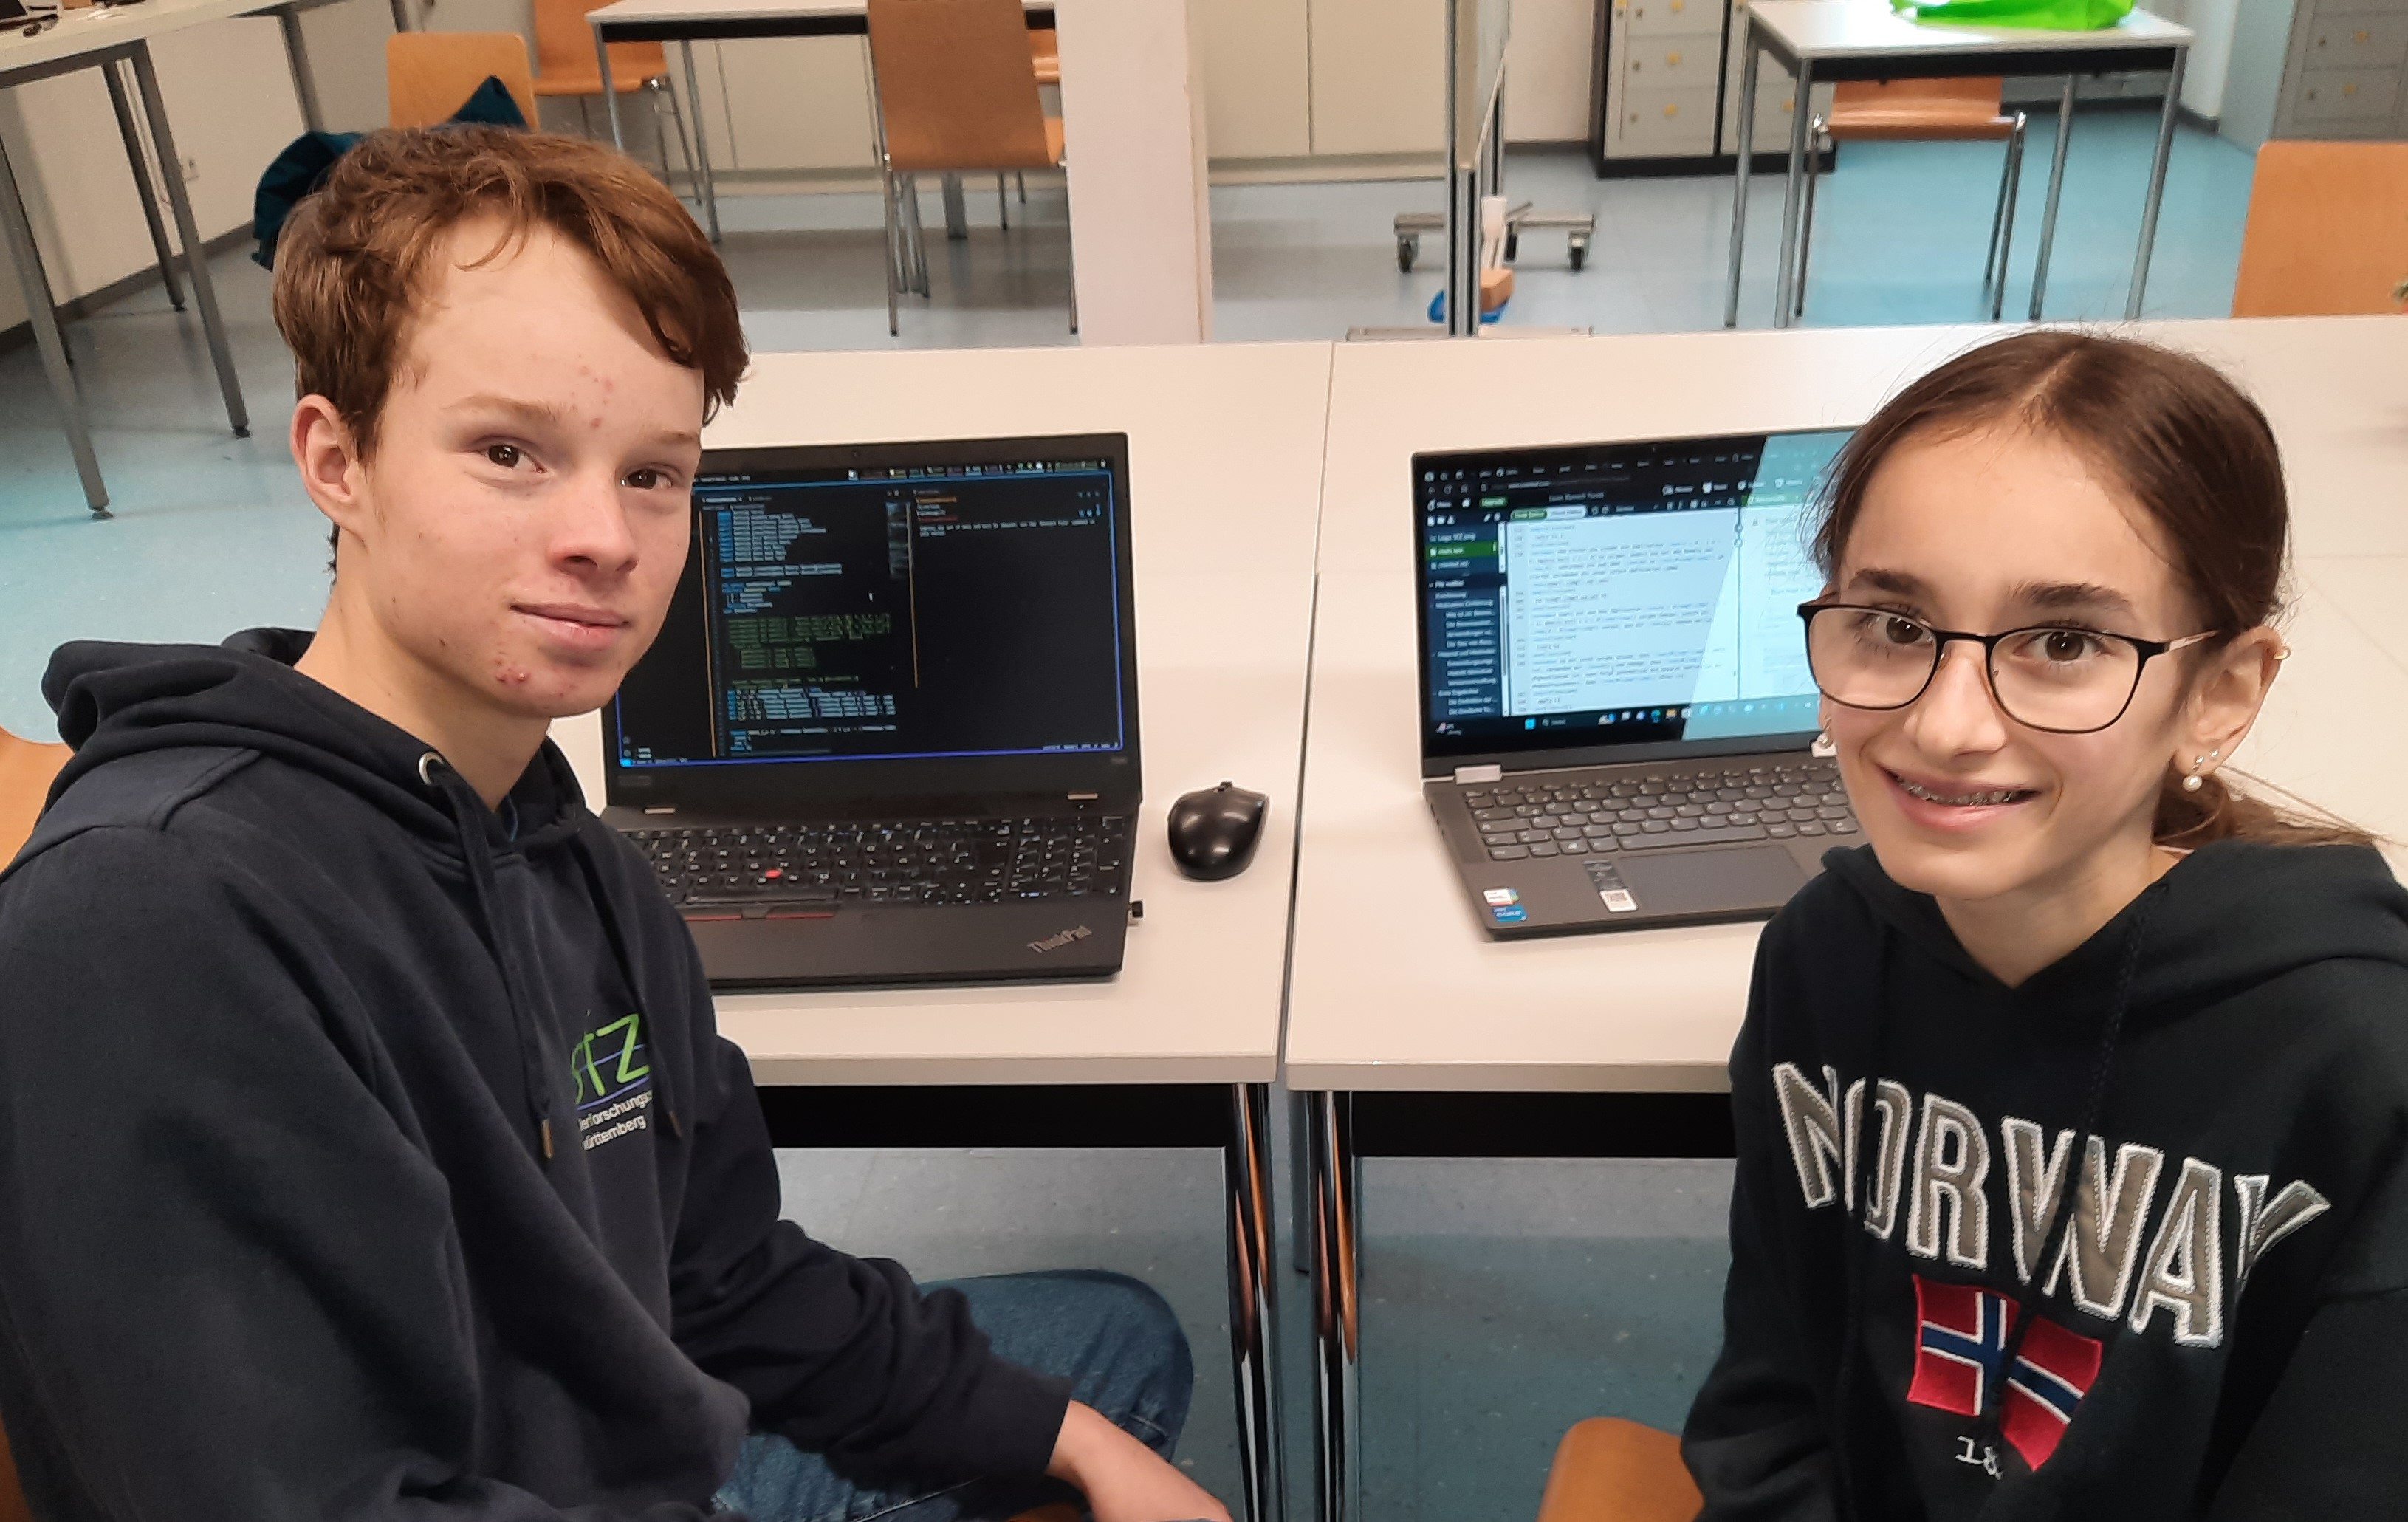
\includegraphics[scale=0.1]{Bild Christian Chiara bearbeitet.jpg}

\end{figure*}
 \begin{center}

 
     \Large\textsc{Chiara Cimino, Otto-Hahn-Gymnasium Tuttlingen\\Christian Krause, Gymnasium Ochsenhausen}\\\vspace{1cm}

    Schülerforschungszentrum Südwürttemberg e.V.\\Standorte Tuttlingen und Ochsenhausen  \vspace{1.5cm}

     \today

 \end{center}~
 \clearpage
 
% \maketitle
\tableofcontents
\listoffigures
\thispagestyle{empty}
%\section*{Kurzfassung}
%Die Forschung in der Mathematik ist eine höchst aktive Welt. Das Herzstück dabei sind die mathematischen Sätze und deren Beweise. Diese Beweise werden aber immer komplizierter und auch die Kontrolle auf Korrektheit ist schwierig und fehleranfällig.\\

%\noindent Da die Verifikation eines Beweises ein nur bedingt kreativer Prozess ist, kann er in sogenannten Beweisassistenten formalisiert werden. Lean in der Version 3 und 4 ist einer der Modernsten und Leistungsfähigsten. Dies wurde unter anderem durch die Verifikation eines Satzes des deutschen Fields-Medallienträger Peter Scholze sowie an einem Beweis von Terence Tao, ebenfalls Fields-Medallienträger, nachgewiesen.\\

%\noindent In unserem Projekt haben wir uns intensiv mit dem auf Typentheorie basierenden Lean 4 beschäftigt und eigene Definitionen und Beweise „geleant“. Unser großes Ziel ist es, am Ende das Paradoxon von Banach-Tarski, das noch nicht geleant ist, zu leanen und damit einen Beitrag zur Bibliothek der mit Lean verifizierten Sätze zu leisten.


\clearpage

\setcounter{page}{1}
\section{Motivation} %/Einführung}
Die Forschung in der Mathematik ist eine aktive und sehr lebendige Welt. Weltweit wurden vom Fachbereich Mathematik seit 1996 insgesamt 4,5 Millionen Dokumente publiziert. Davon sind rund 300 000 alleine im Jahr 2022 entstanden. Das entspricht einem Anstieg von rund 10\% im Vergleich zum Vorjahr \cite{Q1}. All diese Aufsätze und ihre enthaltenden Beweise müssen selbstverständlich auch auf Korrektheit geprüft werden und mit den stetig steigenden jährlichen Veröffentlichungszahlen gibt es immer mehr zu kontrollieren. Dies ist schwierig, zumal ein auf einem fehlerhaften Resultat aufbauender Beweis ebenfalls ungültig ist. Da mathematische Beweise aber nichts anderes als formale Objekte sind, ist die Idee naheliegend, einen Beweisassistenten zu entwickeln, mit dessen Hilfe Beweise diverser mathematischer Theoreme, Lemmata o.ä. schnell formalisiert und zweifelsfrei verifiziert werden können. 

\noindent Diese Beweisassistenten gibt es schon sehr lange, aber erst in jüngster Zeit, auch mit dem Aufkommen der KI, sind die Möglichkeiten geradezu explodiert und renommierteste Lehrstühle und Professoren sind involviert. \glqq  Formale Beweisassistenten ermöglichen eine Zusammenarbeit in wirklich großem Ausmaß\grqq. Dieses Zitat stammt von dem Mathematiker und Fields-Medallienträger Terence Tao aus seinem Vortrag \glqq Machine assisted proofs\grqq~vom 3. Januar 2024. Es hat sich eine Lean-Community gebildet, die hier intensivst forscht und große Schritte nach vorne macht. Auch wenn wir noch sehr jung sind, wollen wir ein Teil dieser Lean-Community werden. Uns haben die Gedanken fasziniert und wir haben uns zum Ziel gesetzt einen Teil in der Mathlib Bibliothek der maschinell überprüften Beweise beizutragen und so an einer ganz kleinen Stelle als Autoren verewigt zu werden.\par
% RUF: Den Teil habe ich komplett umgeschrieben und natürlich etwas übertrieben, Zur Not wieder zurck drehen...  

\subsection{Was ist ein Beweisassistent?}
% Kommentar RUF: Das Zitat war in der Version hier ziemlich verloren und nicht eingebunden. Daher habe ich es nach oben gepackt 

\noindent Ein mathematischer Beweisassistent ist eine Software, die über eine Programmiersprache verfügt, welche es dem Benutzer erlaubt, mathematische Objekte zu definieren. Ausgehend von diesen Objekten können dann unter Verwendung der zugrunde liegenden Programmiersprache die zugehörigen Eigenschaften, inklusive Beweis, formalisiert werden. Der Beweisassistent kontrolliert ausgehend von seiner logischen Basis die Standhaftigkeit des Beweises und markiert gegebenenfalls Fehler. Diese Basis kann sich allerdings von Assistent zu Assistent unterscheiden. 

\subsection{Der Beweisassistent Lean}
Seit 2013 hat sich zu den wenigen bereits existierenden mathematischen Beweisassistenten der Beweisassistent namens Lean gesellt. Das Prinzip von Lean wurde von Leonardo de Moura, damals Microsoft-Mitarbeiter, entwickelt. Mittlerweile ist Lean ein Open Source Project, dass von der Community weiterentwickelt wird.\par

\begin{minipage}{6cm}
\begin{figure}[H]
    \centering
    
\includegraphics[scale=0.20]{Lean Logo.jpg}
    \label{Abb1}
    \caption{Lean Logo \cite{Q12}}
    
\end{figure}
\end{minipage}
\begin{minipage}{10cm}
Die aktuellste Version von Lean (Lean4) ermöglicht die Kontrolle von Beweisen in fast allen Teilgebieten der Mathematik auf Basis der sogenannten Typentheorie. Die erste offizielle Version von Lean4 wurde erst im September 2023 veröffentlicht \cite{Q2}, was Lean zu einem der aktuellsten Beweisassistenten macht.
\end{minipage}

\noindent Bereits in Lean formalisierte mathematische Theoreme werden in einer allgemein zugänglichen Bibliothek, genannt Mathlib Bibliothek, gespeichert. Die Aussagen dieser Sätze können dann ohne einen weiteren Beweis vorausgesetzt werden und bei dem Formalisieren von neuen Sätzen inkl. Beweis verwendet werden. Aufgrund des jungen Alters von Lean umfasst diese Bibliothek aber noch lange nicht den aktuellen Stand der mathematischen Forschung und es sind viele Lücken vorzufinden. \cite{Q8}\par
% TODO ggf. gesamte Erklärung zu Mathlib hier

\noindent Das wohl bekannteste Beispiel ist die Formalisierung des von dem deutschen Fields-Medallienträger Peter Scholze aufgestellten Liquid Tensor Experiments in Lean. Durch Lean konnten mehrere kleinere Ungenauigkeiten in seinem Beweis gefunden und korrigiert werden. Außerdem konnten an einzelnen Stellen Vereinfachungen gefunden werden und im Juli 2022 wurde die Verifizierung des Liquid Tensor Experiments abgeschlossen \cite{Q13}. Es ist erstaunlich, dass Lean diesen Beweis verifizieren konnte, da selbst Peter Scholze Zweifel hatte (\glqq I think nobody else has dared to look at the details of this, and so I still have some small lingering doubts\grqq; Peter Scholze, Dezember 2020) und bis dahin fast niemand das Liquid Tensor Experiment vollständig durchdringen konnte. 

\noindent Das ist auch der Grund, weshalb sich Mathematikerinnen und Mathematiker weltweit vernetzen, um weitere Sätze in Lean zu formalisieren. Unser Team ist, wie gesagt, nun eines der jüngsten Mitglieder dieser Community, denn uns hat diese Fortschrittlichkeit und das vielfältige Netzwerk der Lean-Community fasziniert. \\

\subsection{Das Paradoxon von Banach-Tarski}\label{1.3}
Auf der Suche nach einem spannenden und alltagsnahen mathematischen Satz, der noch nicht in der sogenannten Mathlib Bibliothek ist, sind wir auf den Satz von Banach-Tarski gestoßen, auch bekannt als Banach-Tarski-Paradoxon.
\vspace*{-0.8cm}
\begin{figure}[H]
    \centering
    
\includegraphics[scale=0.15]{Bild Banach Tarski.png}
    \label{Abb2}
    \caption{Anschauliche Darstellung der Hauptaussage von Banach-Tarski \cite{Q11} }
    
\end{figure}
\vspace{-0.2cm}
\noindent Dieser besagt, dass die Einheitskugel in eine endliche Anzahl an Teilen zerlegt werden kann, welche neu angeordnet zwei Kopien der ursprünglichen Einheitskugel ergeben. Dies ist entgegen aller anfänglichen Intuition, da Verschiebungen und Drehungen im euklidischen Raum bekanntlich volumenerhaltend sind. Es ist aber zu erwähnen, dass dieser Volumenbegriff nur bei sog. messbaren Mengen sinnvoll ist. Im Satz von Banach-Tarski wird die Einheitskugel aber in nicht Lebesgue-messbare Mengen zerlegt. Die Existenz solcher nicht Lebesgue-messbaren Mengen folgt mit dem Auswahlaxiom.

\noindent Auf den Punkt gebracht folgt also mit dem Satz von Banach-Tarski unter bestimmten Rahmenbedingungen: \glqq Aus eins mach zwei durch zerschneiden, drehen und wieder zusammen setzen\grqq.

\section{Material und Methoden}

\subsection{Entwicklungsumgebung}
Als Entwicklungsumgebung verwenden wir VS Code in Kombination mit dem Lean4 Plugin \cite{Q3}. Dieses implementiert einen Language Server, der die Lean Programme in Echtzeit kompiliert und auf Fehler überprüft. Außerdem werden in einem Fenster neben dem Programm Informationen, z.B. zu dem aktuellen Theorem angezeigt.
\begin{figure}[H]
    \centering
    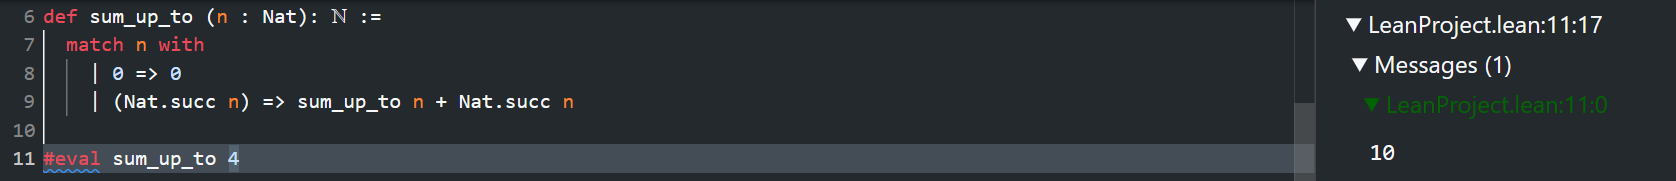
\includegraphics[width=0.95\linewidth]{Abbildung sum_up_to.png}
    \caption{Die sum\_up\_to Funktion in VS Code}
    \label{Abb sum_up_to}
\end{figure}
\vspace{-0.2cm}
\noindent In Abbildung \ref{Abb sum_up_to} sieht man exemplarisch, wie das Lean4 VS Code Plugin bestimmte Syntax Elemente farblich hervorhebt. Außerdem wird das Ergebnis des Befehls \lean/#eval sum_up_to 4/ direkt berechnet und in dem Fenster rechts angezeigt.
\vspace{-0.2cm}
\hspace{-0.4cm}
\begin{figure}[H]
    \centering
    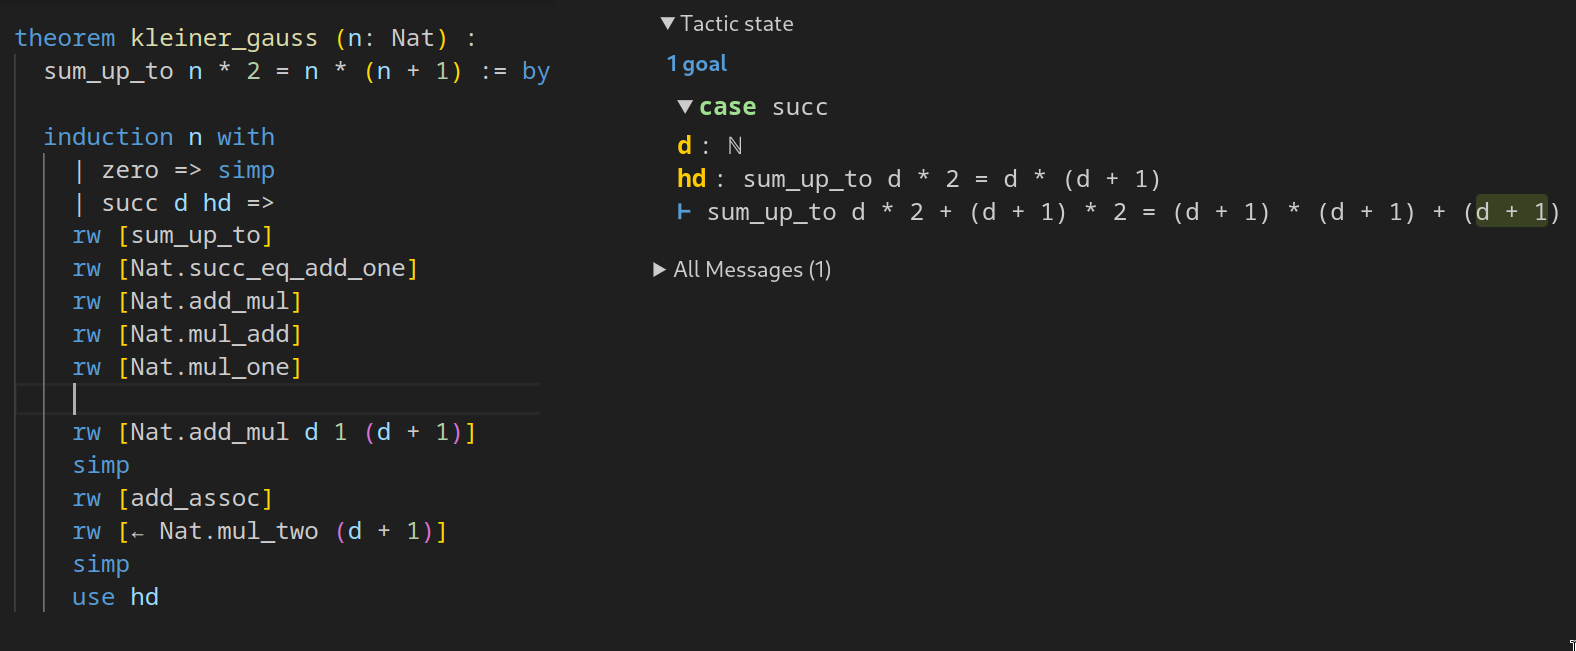
\includegraphics[width=0.65\linewidth]{kleiner_gauss.png}
    \caption{Enter Caption}
    \label{Abb Enter Caption}
\end{figure}
\noindent Die Anzeige des Lean Plugins während eines Beweises ist beispielhaft in Abbildung \ref{Abb Enter Caption} zu erkennen. Es wird der Zwischenstand des Beweises an der Position des Cursors angezeigt. Das ist vor allem bei Beweisen, die mit Taktiken arbeiten, hilfreich.

\subsection{Mathlib Bibliothek}
Eines der großen Ziele von Lean ist es, alle Beweise der Mathematik zu formalisieren und so zu überprüfen. Davon ist die Lean-Community zwar noch weit entfernt, aber es sind bereits viele grundlegende mathematische Theoreme und Lemmata aus vielen verschiedenen Bereichen in Lean implementiert. Diese Theoreme und Lemmata sind in der Mathlib \cite{Q10} katalogisiert und können so auch in darauf aufbauenden Beweisen verwendet werden. Die Mathlib wurde ursprünglich in einer älteren Lean3-Version verfasst, ist aber mittlerweile vollständing in Lean4 übersetzt. Außerdem ist sie frei zugänglich, d. h. jeder kann sie in eigenen Lean Projekten verwenden und auch Erweiterungsvorschläge machen.

\subsection{Blueprint}



%&(Quellen oder Beispiel angeben: PFR und Liquid Tensor experiment (https://leanprover-community.github.io/liquid/index.html)) 

TODO Ziel: PR zu offziellem Blueprint repo

\subsection{Versionsverwaltung}
Wir speichern die Versionen von unseren Lean Programmen in einem Git Repository, das auch auf Github zu finden ist. Git ist der Standart für Versionsverwaltung von größeren Informatikprojekten, die Mathlib verwendet ebenfalls git und ist auf Github hochgeladen.

\section{Erste Ergebnisse und wie man mit Lean arbeitet}
Bevor wir uns an das Leanen des Banach-Tarski-Paradoxons machten, fangen wir mit kleineren Beispielen an; zunächst mal, um die Arbeitsweisen von Lean zu verstehen. Diese von uns selbst \glqq geleanten\grqq~Beispiele wollen wir dem Leser in den folgenden Unterkapiteln vorstellen, damit man sich selber ein Bild machen kann.  

\subsection{Der \glqq kleine Gauß\grqq; Verifikation des Beweises mit Lean}
\noindent Auch hier besteht die Möglichkeit, zum besseren Verständnis des Beweises durch folgenden Link auf das
original Lean-Dokument zuzugreifen: \href{https://live.lean-lang.org/#code=import%20Mathlib.Data.Nat.Basic%0D%0Aimport%20Mathlib.Data.Real.Basic%0D%0A%0D%0Adef%20CC_sum_up_to%20(n%20%3A%20Nat)%3A%20%E2%84%95%20%3A%3D%0D%0A%20%20match%20n%20with%0D%0A%20%20%20%20%7C%200%20%3D%3E%200%0D%0A%20%20%20%20%7C%20(Nat.succ%20n)%20%3D%3E%20CC_sum_up_to%20n%20%2B%20Nat.succ%20n%0D%0A%0D%0A%23eval%20CC_sum_up_to%204%0D%0A%0D%0A%0D%0A%0D%0Atheorem%20CC_kleiner_gauss%20(n%3A%20Nat)%20%3A%0D%0A%20%20CC_sum_up_to%20n%20*%202%20%3D%20n%20*%20(n%20%2B%201)%20%3A%3D%20by%0D%0A%0D%0A%20%20induction%20n%20with%0D%0A%20%20%20%20%7C%20zero%20%3D%3E%0D%0A%20%20%20%20simp%0D%0A%20%20%20%20rw%20%5BCC_sum_up_to%5D%0D%0A%20%20%20%20%7C%20succ%20d%20hd%20%3D%3E%0D%0A%20%20%20%20rw%20%5BCC_sum_up_to%5D%0D%0A%20%20%20%20rw%20%5BNat.succ_eq_add_one%5D%0D%0A%20%20%20%20rw%20%5BNat.add_mul%5D%0D%0A%20%20%20%20rw%20%5BNat.mul_add%5D%0D%0A%20%20%20%20rw%20%5BNat.mul_one%5D%0D%0A%0D%0A%20%20%20%20rw%20%5BNat.add_mul%20d%201%20(d%20%2B%201)%5D%0D%0A%20%20%20%20simp%0D%0A%20%20%20%20rw%20%5Badd_assoc%5D%0D%0A%20%20%20%20rw%20%5B%E2%86%90%20Nat.mul_two%20(d%20%2B%201)%5D%0D%0A%20%20%20%20simp%0D%0A%20%20%20%20exact%20hd}{live-lean.kleiner.gauß}\par
\vspace{0.2cm} 
\noindent Da der wesentliche Teil dieses Programms aber das Kontrollieren von Beweisen ist, dreht sich nun dieses Kapitel um das Codieren des Beweises einer der bekanntesten Formeln: Der Gaußschen Summenformel oder besser bekannt, als der \glqq kleine Gauß\grqq. Diese ermöglicht die Berechnung der Summe der ersten $n$ natürlichen Zahlen.

\noindent Bevor es nun an unseren ersten Satz geht, benötigen wir aber vorab noch eine Definition, welche uns folgende Summe für $n\in \mathbb{N}_0$ definiert: $\sum_{k=0}^{n}k$. Diese Summe haben wir wie folgt definiert:
\begin{leancode}
def CC_sum_up_to (n : Nat): ℕ :=
  match n with
    | 0 => 0
    | (Nat.succ n) => CC_sum_up_to n + Nat.succ n
\end{leancode}
Um die Summe allgemein definieren zu können, führen wir am Anfang unserer Definition eine Variable \lean/n/ ein, welche vom Typ $\mathbb{N}$ ist. Hierbei ist zu erwähnen, dass Lean $0$ in diesem Fall als eine natürliche Zahl auffasst.\par
\noindent Da wir das Ganze über eine Zuordnung definieren möchten, müssen wir selbstverständlich auch unseren Wertebereich angeben, was wir durch \lean/: ℕ/ erreichen. Dies heißt, dass unser Funktionswert ebenfalls vom Typ der natürlichen Zahlen ist.

\noindent Mit \lean/match n with/ machen wir Lean klar, dass es sich hier um eine Zuordnung handelt, wobei \lean/n/ unser Ausgangswert ist.\par

\noindent In den folgenden beiden Zeilen Code definieren wir die Abbildungsvorschrift induktiv. Da Lean $0$ als natürliche Zahl auffasst, ist unser Induktionsanfang hier $0$, statt $1$.\par

\noindent Die letzte Zeile beinhaltet unseren Induktionsschritt. Bzgl. der Begriffsklärung ist zu sagen, dass \lean/Nat.succ n/ die Notation für die Zahl $n+1$ ist, wenn $n\in \mathbb{N}_0$ gilt.

\noindent Um zu kontrollieren, dass unsere Definition das Gewünschte liefert, können wir Lean für \lean/n/ eine bestimmte Zahl einsetzen lassen bspw. $5$. Dann erhalten wir in unserer Kontrolleiste rechts folgende Statusmeldung:
\begin{figure}[H]
    \centering
    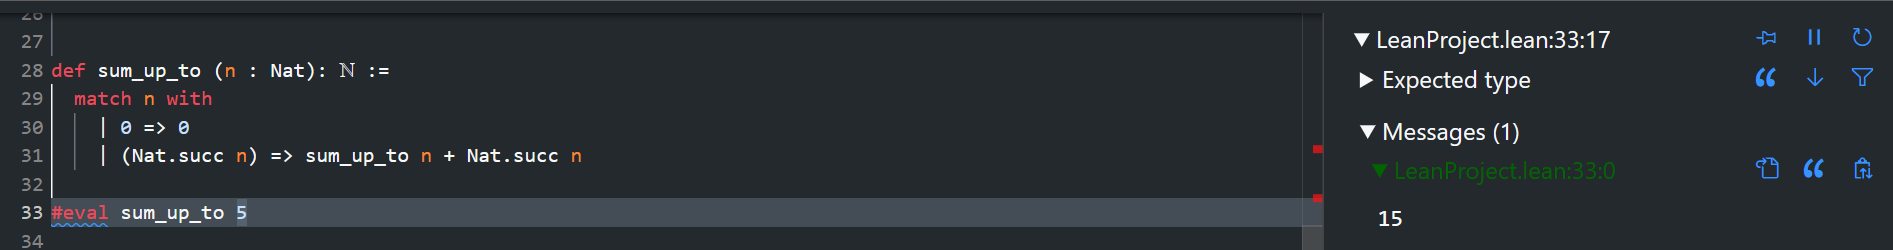
\includegraphics[scale=0.5]{sum_up_to 5.png}
    \label{Abb2}
    \caption{Test von \lean/sum_up_to/}
    
\end{figure}
\noindent Hierfür verwenden wir die Funktion \lean/eval/, welche hier $5$ nach den definierten Zuordnungsvorschriften dem entsprechendem Wert zuordnet. Dass $15$ das korrekte Ergebnis der Summe ist, kann man schnell nachrechnen.

\noindent Nachdem wir nun $\sum_{k=0}^{n}k$ für ein $n\in \mathbb{N}_0$ definiert haben, können wir nun unser Theorem formalisieren:
\begin{leancode}
theorem CC_kleiner_gauss (n: Nat) : CC_sum_up_to n * 2 = n * (n + 1) := by
\end{leancode}
Auf die Benennung des Theorems folgt sogleich die Voraussetzung \lean/(n: Nat)/, was bedeutet, dass \lean/n/ den Typ der natürlichen Zahlen hat. Nach dem zweiten Doppelpunkt folgt unsere Behauptung: $$\sum_{k=0}^{n}k=\frac{n\cdot (n+1)}{2} 
~\textbf{oder}~2\cdot\sum_{k=0}^{n}k=n\cdot (n+1)$$
\noindent Diese Umformung erleichtert uns später den Beweis. Die obige Gleichheit formalisieren wir in Lean mithilfe von \lean/CC_sum_up_to/. \lean/:= by/ kennzeichnet, dass die nachfolgende Zeile den Beweis der vorausgehenden Behauptung einläutet.

\noindent Sprechen wir schon von dem Beweis, so ist zu erwähnen, dass beim Beweisen in Lean verschiedene Taktiken verwendet werden. Die wohl von uns am meisten verwendete Taktik ist die \glqq rewrite\grqq~(kurz: \lean/rw/) Taktik. Diese Taktik wird verwendet falls wir ein Beweis h eines Ausdrucks $X=Y$ gegeben haben. Dann erreichen wir durch \lean/rw[h]/, dass alle $X$ im noch zu zeigenden Ziel durch $Y$ ausgetauscht werden. Die \glqq rewrite\grqq~Taktik kann daher insbesondere bei bereits in Lean bewiesenen Axiomen bzgl. Äquivalenzumformung verwendet werden. Dann erreichen wir mit \lean/rw/ und dem Namen des Axioms, dass das zu zeigende Ziel entsprechend des Axioms umgeschrieben wird. Zum Beispiel können wir einen Ausdruck der Form $(a+b)\cdot c$ in unserem Ziel mit \lean/rw[add_mul]/ zu $a\cdot c+b\cdot c$ umschreiben.

\noindent Eine weitere sehr hilfreiche Taktik ist die \lean/simp/ Taktik (kurz für: \glqq simplify\grqq~). Diese vereinfacht das noch zu zeigende Ziel unter Verwendung von \lean/rw/ so weit wie nur möglich. Wir können grundsätzlich nicht alle Umformungen, die wir mit \lean/rw/ durchführen, einfach durch \lean/simp/ ersetzen. \lean/simp/ kann nur sehr grundlegende Umformungen durchführen und ob man mit \lean/simp/ eine sinnvolle Umformung erhält ist situationsabhängig. Ein Versuch ist es aber meistens Wert.\par
\noindent Sollte man mit \lean/simp/ keinen Erfolg haben, so muss mit einer anderen Taktik weiter gearbeitet werden.

\noindent Abgesehen von \lean/rw/ und \lean/simp/ gibt es noch \lean/exact/. Diese Taktik verwenden wir genau dann, wenn wir allgemein eine Aussage, nennen wir sie $P$, nach dem Vereinfachen unserer Behauptung noch zu zeigen haben, wobei ein Beweis $h$ dieser Aussage $P$ in Lean schon gegeben ist. \lean/exact h/ sagt Lean dann, dass es den Beweis $h$ verwenden soll, womit dann der Beweis abgeschlossen wird.\\

\noindent Kommen wir nun also wieder auf unser ursprüngliches Theorem, der Gültigkeit der Gaußschen Summenformel für alle natürlichen Zahlen, inklusive der Null, zurück, so erhalten wir nur durch die Verwendung der oben vorgestellten Taktiken folgenden Beweis:
\begin{leancode}
theorem CC_kleiner_gauss (n: Nat) : CC_sum_up_to n * 2 = n * (n + 1) := by
  induction n with
    | zero => 
    simp
    rw [CC_sum_up_to]
    | succ d hd => 
    rw [CC_sum_up_to]
    rw [Nat.succ_eq_add_one]
    rw [Nat.add_mul]
    rw [Nat.mul_add]
    rw [Nat.mul_one]
    rw [Nat.add_mul d 1 (d + 1)]
    simp
    rw [add_assoc]
    rw [← Nat.mul_two (d + 1)]
    simp
    exact hd
\end{leancode}
\noindent Wie man gut erkennen kann, haben wir den Beweis mithilfe einer Induktion über \lean/n/ aufgestellt. Wir haben daher zunächst Folgendes zu zeigen: \lean/CC_sum_up_to Nat.zero * 2 = Nat.zero * (Nat.zero + 1)/. Die Taktik \lean/simp/ formt das Ziel zu \lean/CC_sum_up_to 0 = 0/ um. Nun können wir die Definition von \lean/CC_sum_up_to/ verwenden und damit den Beweis für \lean/n=0/ abschließen.

\noindent Anschließend gehen wir zum Induktionsschritt über, in dem wir voraussetzen, dass die Gleichheit für eine natürliche Zahl $d$ gilt. Diese Voraussetzung betiteln wir hier mit \lean/hd/. Dann zeigen wir, dass die Behauptung auch für $d+1$ wahr ist. Hierfür schreiben wir unser Ziel zunächst mit unserer eigenen Definition \lean/CC_sum_up_to/ um. Anschließend verwenden wir unter der Taktik \lean/rw/ eine Reihe an in der Mathlib Bibliothek verfügbaren bereits bewiesen Axiome. Die Namen dieser Axiome verraten schon, wie diese das Ziel umformen werden.

\noindent Damit dennoch keine Unklarheiten entstehen, sind in der folgenden Tabelle die Aussagen der einzelnen Axiome aufgeführt. $a,b$ und $c$ sind hier beliebige natürliche Zahlen.
\begin{center}
\begin{tabular}{| c | c |}
\hline
\lean/Nat.succ_eq_add_one/ &  \lean/Nat.succ a = a+1/\\
\hline
\lean/Nat.add_mul/ & $(a+b)\cdot c=a\cdot c+b\cdot c$\\
\hline
\lean/Nat.mul_add/ & $a\cdot c+b\cdot c=(a+b)\cdot c$\\
\hline
\lean/Nat.mul_one/ & $a\cdot 1=a$\\
\hline
\lean/Nat.add_mul a 1 (a + 1)/ & $(a+1)\cdot (a+1)=a\cdot (a+1)+1\cdot(a+1)$\\
\hline
\lean/add_assoc/ & $(a+b)+c=a+b+c$\\
\hline 
\lean/← Nat.mul_two (a + 1)/ & $a+1+(a+1)=(a+1)\cdot 2$\\
\hline
\end{tabular}
\end{center}
\noindent Nach der chronologischen Verwendung dieser Axiome und nach mehrfachem Vereinfachen mithilfe von \lean/simp/, haben wir noch \lean/CC_sum_up_to d * 2 = d * (d + 1)/ zu zeigen übrig. Dies entspricht aber genau der Aussage von \lean/hd/. Anwenden der Taktik \lean/apply/ in Kombination mit \lean/hd/ liefert dann das gewünschte Ergebnis.\par
\noindent Falls das Bedürfnis besteht, den mathematischen Beweis einzusehen, kann man dies über folgenden Link machen: \href{https://mathedia.com/beweis-der-gaussschen-summenformel/}{kleiner-gauß}


\iffalse % Das nächste Kapitel ist auskommentiert
\subsection{Ein erstes Lemma}
\noindent Auch hier besteht die Möglichkeit, zum besseren Verständnis des Beweises durch folgenden Link auf das Original Lean-Dokument zuzugreifen:
\href{https://live.lean-lang.org/#code=import%20Mathlib.Topology.MetricSpace.Basic%0D%0A%0D%0Avariable%20%7BX%20%3A%20Type*%7D%20%5BMetricSpace%20X%5D%20(M%20%3A%20Set%20X)%0D%0A%0D%0A--%20Definition%20der%20Offenheit%0D%0Adef%20CC_is_open_set%20(M%20%3A%20Set%20X)%20%3A%20Prop%20%3A%3D%0D%0A%20%20%E2%88%80%20x%20%E2%88%88%20M%2C%20%E2%88%83%20%CE%B5%20%3E%200%2C%20Metric.ball%20x%20%CE%B5%20%E2%8A%86%20M%0D%0A%0D%0A--%20Definition%20der%20Abgeschlossenheit%0D%0Adef%20CC_is_closed_set%20(M%20%3A%20Set%20X)%20%3A%20Prop%20%3A%3D%0D%0A%20%20CC_is_open_set%20M%E1%B6%9C%0D%0A%0D%0A%0D%0Atheorem%20CC_compl_compl_eq_set%20(M%20%3A%20Set%20x)%20%3A%20M%20%3D%20M%E1%B6%9C%E1%B6%9C%20%3A%3D%20by%0D%0A%20%20exact%20eq_compl_comm.mpr%20rfl%0D%0A%0D%0A%0D%0A--%20Beweis%2C%20dass%20M%20offen%20ist%2C%20wenn%20und%20nur%20wenn%20M%E1%B6%9C%20abgeschlossen%20ist%0D%0Atheorem%20CC_open_iff_complement_closed%20(M%20%3A%20Set%20X)%20%3A%0D%0A%20%20CC_is_open_set%20M%20%E2%86%94%20CC_is_closed_set%20M%E1%B6%9C%20%3A%3D%20by%0D%0A%20%20rw%20%5Biff_def%5D%0D%0A%0D%0A%20%20have%20h%3A%20CC_is_open_set%20M%20-%3E%20CC_is_closed_set%20M%E1%B6%9C%0D%0A%20%20intro%20h1%20x%0D%0A%20%20rw%20%5Bcompl_compl%5D%0D%0A%20%20intro%20hx%0D%0A%20%20exact%20h1%20x%20hx%0D%0A%0D%0A%20%20have%20k%3A%20CC_is_closed_set%20M%E1%B6%9C%20-%3E%20CC_is_open_set%20M%0D%0A%20%20intro%20k1%20x%0D%0A%20%20rw%20%5BCC_compl_compl_eq_set%20M%5D%0D%0A%20%20intro%20kx%0D%0A%20%20exact%20k1%20x%20kx%0D%0A%0D%0A%20%20exact%20%7B%20left%20%3A%3D%20h%2C%20right%20%3A%3D%20k%20%7D}{live-lean.äquivalenz}\par
\vspace{0.2cm}
\noindent Nachdem wir den Beweis der Gaußschen Summenformel nun erfolgreich in Lean formalisiert haben, nehmen wir uns jetzt ein Lemma aus der Analysis 1 vor, um das Formalisieren in Lean auf das nächst höhere Level zu heben. Wir haben uns hierbei für folgenden Satz entschieden, da wir metrische Räume äußerst spannend finden und dieser Satz sehr vielfältig verwendet werden kann.

\begin{lemma}\label{satz1}
Sei $(X,d)$ ein metrischer Raum. Dann ist $M\subset X$ offen, genau dann, wenn $M^c$ abgeschlossen ist.   
\end{lemma}
\noindent Um diesen Satz zu leanen, benötigen wir zunächst die hierfür notwendigen Software-Pakete. Nach dem Durchforsten der Mathlib Bibliothek stellen sich die folgenden Usepackages als zielführend heraus:
\begin{leancode}
import Mathlib.Topology.MetricSpace.Basic
import Mathlib.Topology.MetricSpace.PseudoMetric
\end{leancode}
\noindent Bevor wir nun das Lemma formalisieren, sind vorab noch Definitionen aufzustellen und damit wir nicht jedes Mal einen metrischen Raum \lean/X/ und eine Teilmenge \lean/M/ von \lean/X/ wählen müssen, definieren wir uns diese zunächst als Variablen:
\begin{leancode}
variable {X : Type*} [MetricSpace X] (M : Set X)
\end{leancode}
\noindent Diese Definition der Variablen wird in die kommenden Definitionen und in das eigentliche Theorem übertragen.

\noindent Um die Äquivalenz aus Lemma \ref{satz1} zu zeigen, müssen wir als erstes aber in Lean definieren, was es bedeutet, wenn \lean/M/ offen bzw. abgeschlossen ist. Hierbei kann man die Definition von abgeschlossenen und offenen Mengen in metrischen Räumen gut wiedererkennen. 
\begin{leancode}
-- Definition der Offenheit
def CC_is_open_set : Prop :=
  ∀ x ∈ M, ∃ ε > 0, Metric.ball x ε ⊆ M
  
-- Definition der Abgeschlossenheit
def CC_is_closed_set : Prop :=
  is_open_set M\compl
\end{leancode}
\noindent \lean/M\compl/ bezeichnet dabei das Komplement von $M$.

\noindent Dass wir für die beiden Definitionen den Typ \lean/Prop/ vorgeben, hat den einfachen Grund, dass wir beide Mengeneigenschaften in der jeweiligen nächsten Zeile über Propositionen definieren. Die Verwendung dieses Typs ermöglicht es uns, die mit der Definition verbundenen Proposition in den kommenden als solche zu verwenden.

\noindent Vor dem endgültigen Start, Lemma \ref{satz1} zu formalisieren, stellen wir uns zuvor noch ein Hilfslemma auf, welches besagt, dass \lean/M=M\compl\compl/ für ein \lean/M : Set X/ gilt.
\begin{leancode}
theorem CC_compl_compl_eq_set (M : Set X) : M = M\compl\compl := by
\end{leancode}
\noindent Um dies zu zeigen, verwenden wir das in Lean schon formalisierte Lemma, welches auf unsere Metrik übertragen besagt, dass für \lean/M N : Set X/ die Äquivalenz \lean/M\compl=N \Leftrightarrow M=N^\compl/ gilt. Dieses Lemma trägt in Lean den Namen \lean/eq_compl_comm.mpr/. In Kombination mit der Taktik \lean/exact/ und verbunden mit \lean/rfl/, womit Lean das noch zu zeigende Ziel so weit wie möglich selbständig vereinfacht, Ist das Hilfslemma dann bewiesen.

\noindent Zusammengefasst sieht der Beweis in Lean dann wie folgt aus:
\begin{leancode}
theorem CC_compl_compl_eq_set (M : Set x) : M = M\compl\compl := by
  exact eq_compl_comm.mpr rfl
\end{leancode}
\noindent Nach diesen Vorbereitungen können wir nun anfangen, Satz \ref{satz1} zu formalisieren.
\begin{leancode}
theorem CC_open_iff_complement_closed :
 CC_is_open_set M ↔ CC_is_closed_set M\compl := by
\end{leancode}
\noindent Da wir eine Äquivalenz zu zeigen haben, zerlegen wir diese zunächst in zwei Implikationen, die wir dann separat zeigen:
\begin{leancode}
  rw [iff_def]
\end{leancode}
\noindent Nun einigen wir uns darauf, zuerst die Implikation \lean/CC_is_open_set M -> CC_is_closed_set M\compl/ zu beweisen:
\begin{leancode}
  have h: CC_is_open_set M -> CC_is_closed_set M\compl 
\end{leancode}
\noindent Hierbei darf man sich nicht von dem Taktiknamen \lean/have/ in die Irre führen lassen. Mit \lean/have/ formalisieren wir uns ein Zwischenziel \lean/CC_is_open_set M -> CC_is_closed_set M\compl/, dass wir \lean/h/ nennen und welches wir in den folgenden Zeilen Code beweisen müssen. Die Taktik bedeutet \underline{nicht}, dass wir die Implikation einfach voraussetzen.\par

\noindent Jetzt haben wir eine Implikation zu zeigen, wofür wir \lean/CC_is_open_set M/ voraussetzen, d.h. wir setzen voraus, dass \lean/M/ eine offene Menge ist. Dies wollen wir mit \lean/h1/ betiteln. Nun müssen wir noch zeigen, dass \lean/M\compl/ abgeschlossen ist und nach der Definition der Abgeschlossenheit, ist dies äquivalent dazu, dass \lean/M\compl\compl/ offen ist. Damit wir also zeigen können, dass \lean/M\compl\compl/ offen ist, müssen wir eine für-alle-Aussage zeigen. Daher wählen wir uns in Verbindung mit \lean/h1/ direkt auch ein \lean/x/ vom Typ \lean/X/. Dies erreichen wir durch folgende Zeile:
\begin{leancode}
  intro h1 x
\end{leancode}
\noindent Wir wollen anschließend den Ausdruck \lean/M\compl\compl/ im Ziel zu \lean/M/ vereinfachen, weshalb wir nun das in Lean bereits formalisierte entsprechende Lemma \lean/compl_compl/ verwenden. Da wir dann immer noch eine Implikation \lean/x ∈ M → ∃ ε > 0, Metric.ball x ε ⊆ M/ zu zeigen haben, setzen wir \lean/x ∈ M/ unter dem Namen \lean/hx/ voraus:
\begin{leancode}
  rw [compl_compl]
  intro hx
\end{leancode}
\noindent Jetzt können wir verwenden, dass \lean/M/ offen ist. Dies haben wir \lean/h1/ genannt:
\begin{leancode}
  apply h1
\end{leancode}
\noindent Da wir nun noch \lean/x ∈ M/ zu zeigen haben, was wir ebenfalls schon in unserer Voraussetzungsleiste als \lean/hx/ stehen haben, verwenden wir dieselbe Taktik mit \lean/hx/:
\begin{leancode}
  apply hx
\end{leancode}
\noindent Nun haben wir $h$ erfolgreich gezeigt. Da wir aber selbstverständlich noch die Implikation in die andere Richtung zeigen müssen, verwenden wir ein weiteres Mal die Taktik \lean/have/:
\begin{leancode}
  have k: CC_is_closed_set M\compl -> CC_is_open_set M
\end{leancode}
\noindent Um diese Implikation zu zerlegen, gehen wir zunächst analog vor, wie bei dem Beweis von \lean/h/. Wir setzen daher voraus, dieses Mal unter dem Namen \lean/k1/, dass \lean/M\compl/ abgeschlossen ist. Da wir nun zeigen müssen, dass \lean/M/ offen ist, greifen wir erneut auf unsere Definition der Offenheit einer Menge zurück und wählen uns daher wieder ein \lean/x/ vom Typ \lean/X/:
\begin{leancode}
  intro k1 x
\end{leancode}
\noindent Nun bleibt uns wieder die Implikation \lean/x ∈ M → ∃ ε > 0, Metric.ball x ε ⊆ M/ zu zeigen. Anders als bei dem Beweis von \lean/h/, schreiben wir nun aber \lean/M/ zu \lean/M\compl\compl/ um. Hierfür verwenden wir unser selbst definiertes Lemma \lean/CC_compl\_compl\_eq\_set/:
\begin{leancode}
  rw [CC_compl_compl_eq_set M] 
\end{leancode}
\noindent Damit wir nun die Implikation \lean/x ∈ M\compl\compl → ∃ ε > 0, Metric.ball x ε ⊆ M\compl\compl/ zeigen können, setzen wir \lean/x ∈ M\compl\compl/ voraus, was wir \lean/kx/ nennen wollen:
\begin{leancode}
  intro kx
\end{leancode}
\noindent Da wir jetzt zeigen müssen, dass \lean/M\compl\compl/ offen ist, verwenden wir \lean/k1/, was besagt, dass \lean/M\compl/ abgeschlossen ist. Dann folgt automatisch mit unserer Definition der Abgeschlossenheit, dass \lean/M\compl\compl/ offen ist:
\begin{leancode}
  apply k1
\end{leancode}
\noindent Nun bleibt noch \lean/x ∈ M\compl\compl/ zu zeigen übrig, wofür wir \lean/kx/ verwenden:
\begin{leancode}
  apply kx 
\end{leancode}
\noindent Damit haben wir auch \lean/k/ gezeigt. Jetzt sind wir nur noch einen kleinen Schritt vom Abschluss des Beweises entfernt.\par

\noindent Da wir unseren Satz in Lean beweisen, bleibt uns noch\par

\noindent \lean/(CC_is_open_set M → CC_is_closed_set M\compl) ∧ (CC_is_closed_set M\compl → CC_is_open_set M)/zu zeigen. Dies erreichen wir durch die Verwendung von \lean/h/ auf der linken Seite sowie durch die Verwendung von \lean/k/ auf der rechten Seite:
\begin{leancode}
  exact { left := h, right := k }
\end{leancode}
\noindent Im Gesamten sieht Lemma \ref{satz1} inkl. Beweis dann wie folgt aus:
\begin{leancode}
theorem CC_open_iff_complement_closed :
  CC_is_open_set M ↔ CC_is_closed_set M\compl := by

  rw [iff_def]
  have h: CC_is_open_set M -> CC_is_closed_set M\compl 
  intro h1 x
  rw [compl_compl]
  intro hx
  apply h1
  apply hx
  have k: CC_is_closed_set M\compl -> CC_is_open_set M
  intro k1 x
  rw [CC_compl_compl_eq_set M] 
  intro kx
  apply k1
  apply kx
  exact { left := h, right := k }
\end{leancode}
\fi % Ende des auskommentierten Teils

\section{Das Banach-Tarski-Paradoxon in Lean}
Nachdem wir uns und den Leser durch kleinere Einheiten mit den Prinzipien von Lean vertraut gemacht haben, wollen wir nun einen komplexeren Satz als Erste überhaupt leanen und dies in einem späteren Schritt in die Mathlib Bibliothek aufnehmen lassen.

\subsection{Mathematischer Hintergrund mit Beweisskizze}

\noindent Die bereits in Kapitel \ref{1.3} informell vorgestellte Herangehensweise, wie man aus einer Kugel zwei mit dem selben Radius der Ausgangskugel erhält, wollen wir nun im mathematischen Licht betrachten.

\noindent Eine wesentliche Rolle spielt dabei eine freie Gruppe $G$, welche von zwei Erzeugern erzeugt wird. Diese sind in diesem Fall Drehwinkel bzw. die zugehörigen Drehmatrizen, welche wir im Folgenden $A$ und $B$ nennen. $G$ soll dabei mit der Gruppenoperation der Konkatenation ausgestattet sein.\par

\noindent Des Weiteren sprechen wir im Folgenden von $A^{-1}$ und $B^{-1}$. $A^{-1}$ kennzeichnet dabei das inverse Element von $A$, d. h. wenn man einen Vektor $(x_1,x_2,x_3)\in\mathbb{R}^3$ zuerst um $A$ dreht und anschließend um $A^{-1}$, so erhält man wieder den ursprünglichen Vektor $(x_1,x_2,x_3)$. Analog definieren wir $B^{-1}$.

\noindent Da wir über $G$ mit der Konkatenation operieren, können wir jedes Element von $G$ als Wort mit den sog. Buchstaben $A, B, A^{-1}$ und $B^{-1}$ darstellen. Dementsprechend ist jedes Element in $G$ eine Hintereinanderausführung der Drehungen $A, B, A^{-1}$ und $B^{-1}$. Damit man sich dies besser vorstellen kann, machen wir zunächst ein Beispiel. Wir wählen hierfür ein Wort $W=[ A^{-1}BAB^{-1} ]$. Wollen wir also einen Vektor $(x_1,x_2,x_3)\in\mathbb{R}^3$ um $W$ drehen, so ist dies äquivalent dazu, dass wir ihn zuerst um $A^{-1}$, dann um $B$, dann um $A$ und anschließend um $B^{-1}$ rotieren.

\noindent Da wir hier von einer freien Gruppe sprechen, ist jedes Wort in $G$ gekürzt, d. h., dass in jedem Wort $[ AA^{-1} ]$, $[ BB^{-1} ]$, $[ A^{-1}A ]$ und $[ B^{-1}B ]$ raus gekürzt sind und diese Kombinationen somit in $G$ nicht vorkommen.\par

\noindent Natürlich soll es uns auch möglich sein, einen Vektor aus dem $\mathbb{R}^3$ nicht zu drehen. Dieses \glqq leere\grqq~Wort notieren wir hier mit $e$.

\noindent Nun unterteilen wir alle Wörter in $G$ in fünf Mengen. Die Menge $S(A)$ beinhaltet alle Wörter, die mit $A$ enden, d. h. man dreht als letztes um $A$. Analog definieren wir uns auch die Mengen $S(A^{-1})$, $S(B)$ und $S(B^{-1})$. Die einelementige Menge $\{e\}$ bildet die letzte Menge. Damit gilt nun $G=S(A)\cup S(A^{-1})\cup S(B)\cup S(B^{-1})\cup \{e\}$

\noindent Die Idee ist nun, die Menge $S(A^{-1})$ um $A$ und die Menge $S(B^{-1})$ um $B$ zu \glqq drehen\grqq. Das soll heißen, dass wir an jedes Wort aus $S(A^{-1})$ $A$ und dementsprechend an jedes Wort aus $S(B^{-1})$ $B$ anhängen. Diese \glqq gedrehten\grqq~Mengen notieren wir mit $S(A^{-1})A$ und $S(B^{-1})B$. Da sich aber $[ A^{-1}A ]$ und $[ B^{-1}B ]$ raus kürzen, entspricht nun die Menge $S(A^{-1})A$ der Vereinigung der Mengen $S(A^{-1})$, $S(B)$ und $S(B^{-1})$, da durch das Anhängen von $A$ das letzte Element $A^{-1}$ aller Elemente in $S(A^{-1})$ eliminiert wurde. $S(A)$ ist in diese Vereinigung nicht mit eingeschlossen, da die Wörter in $G$ bekanntlich alle reduziert sind. Hätte ein Wort $W$ aus $S(A^{-1})$ $A$ als zweitletzten Eintrag, so würden sich $[ AA^{-1} ]$ raus kürzen und damit wäre $W$ nicht mehr in $S(A^{-1})$ enthalten.\par

\noindent Entsprechend gleicht nun $S(B^{-1})B$ der Vereinigung der Mengen $S(B^{-1})$, $S(A)$ und $S(A^{-1})$.

\noindent Damit erhalten wir nun: 
\begin{align*}\label{Eq1}
 G=S(A)\cup S(A^{-1})A\\
 G=S(B)\cup S(B^{-1})B   
\end{align*}
\noindent Hierbei ist zu erwähnen, dass in beiden Gleichungen $\{e\}$ nun überflüssig geworden ist, da $e$ bereits in $S(A^{-1}A$ und $S(B^{-1})B$ enthalten ist. Das liegt daran, dass in $S(A^{-1})$ das Wort $[ A^{-1} ]$ enthalten ist, was wenn $A$ angehängt wird sich zu $e$ kürzt. Analog gilt dies auch bei $S(B^{-1})$ 

\noindent Insbesondere haben wir nun vier der ursprünglichen fünf Mengen zu zwei identischen Kopien der Gruppe zusammengefügt.

\noindent Mit zwei Kopien der freien Gruppe $G$ ist es aber noch nicht getan. Wir wollen nun die Einheitskugel verdoppeln, weshalb wir die Drehungen aus $G$ auf die Punkte der Einheitskugel anwenden. Hierfür beginnen wir mit der Einheitsspähre $L$.\par

\noindent Drehen wir nun einen Punkt $p\in L$ um alle Rotationen, die in $G$ enthalten sind, so bezeichnen wir die Menge aller Punkte, die wir dadurch erhalten, als Bahn von $p$. Anschaulich kann man sich diese als eine kugelförmige Punktwolke vorstellen. Alle somit erhaltenen Bahnen sind paarweise disjunkt und die Vereinigung eben dieser ergibt wieder $L$.

\noindent Das Auswahlaxiom erlaubt uns nun, aus jeder erzeugten Bahn einen Repräsentanten auszuwählen. Wir bezeichnen die Menge aller Repräsentanten mit $R$. Anschließend konstruieren wir uns die Mengen $S(A)R$, $S(A^{-1})R$, $S(B)R$ und $S(B^{-1})R$. $S(A)R$ kennzeichnet hier die Menge aller Punkte, die wir erhalten, wenn wir alle in $R$ enthaltenen Punkte jeweils um alle in $S(A)$ zusammengefassten Drehungen rotieren. Analog sind $S(A^{-1})R$, $S(B)R$ und $S(B^{-1})R$ definiert.

\noindent Grob gesagt können wir die Sphäre $L$ nun unter Verwendung von $S(A)R$, $S(A^{-1})R$, $S(B)R$ und $S(B^{-1})R$ ähnlich wie bei unserer Gruppe $G$ zerlegen und wieder zusammen setzen. Aus dieser Zerlegung der Sphäre folgt dann auch die Zerlegung der Kugel, in dem wir einfach jeden Punkt der Sphäre und jeden Punkt der Mengen $S(A)R$, $S(A^{-1})R$, $S(B)R$ und $S(B^{-1})R$ mit ihrem Ortsvektor ausstatten.\par

\noindent Somit haben wir also unsere Kugel verdoppelt!

\noindent Dass der formale Beweis etwas mehr ins Detail geht ist klar, jedoch führen wir diesen aus Platzgründen nicht vollständig auf. Wer sich für den vollständigen Beweis des Banach-Tarski-Paradoxons im dreidimensionalen Raum interessiert, der kann hier (\cite{Q7}) eine Version einsehen. Damit der Leser aber das folgende Kapitel versteht, wollen wir auf die durch zwei unabhängige Winkel erzeugte Gruppe, mit der wir arbeiten näher eingehen. Das ein solches Winkelpaar existiert, zeigen wir konstruktiv. Hierfür wählen wir uns den Winkel $arccos(\frac{1}{3})$. Wir definieren uns nun $A$ als die Drehmatrix zum Drehwinkel $arccos(\frac{1}{3})$ um die x-Achse und $B$ als die Drehmatrix zum selben Winkel um die z-Achse.\par
\noindent Damit gilt: $A=\frac{1}{3}
\begin{pmatrix}
    3 & 0 & 0 \\
    0 & 1 & -2\sqrt{2} \\
    0 & 2\sqrt{2} & 1 
\end{pmatrix}$, $B=\frac{1}{3}
\begin{pmatrix}
    1 & -2\sqrt{2} & 0 \\
    2\sqrt{2} & 1 & 0 \\
    0 & 0 & 3
\end{pmatrix}$

\noindent Wir können zudem nicht einfach voraussetzen, dass die von $A$ und $B$ erzeugte Gruppe $G$ frei ist. Dies müssen wir beweisen. Um diesen Beweis zu ermöglichen zeigen wir aber zunächst folgendes Lemma:
\begin{lemma}\label{lemma1}
    Sei $\rho : \mathbb{R}^3 \rightarrow \mathbb{R}^3$ ein Ausdruck in $G$ von der Länge $n$ in reduzierter Form. Dann hat $\rho (0,1,0)$ die Form $\frac{1}{3^n}(a\sqrt{2},b,c\sqrt{2})$, wobei $a,b$ und $c$ ganze Zahlen sind.
\end{lemma}
\noindent Das $\rho$ in diesem Lemma ist somit eine Abbildung, die einem Punkt aus dem $\mathbb{R}^3$, den Punkt zuordnet, den man erhält, wenn man diesen Punkt durch ein zugehöriges Element $W$ in $G$ dreht. $W$ ist dabei ein Wort von der Länge $n$ und bereits reduziert.\par


\subsection{Umsetzung in Lean}
\noindent Wie bei dem \glqq kleinen Gauß\grqq~und der Definition der komplexen Zahlen in Lean, gibt es auch für diesen Satz einen Live-Lean-Link, um die einzelnen Schritte besser nachvollziehen zu können: 
\href{https://live.lean-lang.org/#code=import%20Mathlib.Tactic%0D%0Aimport%20Mathlib.GroupTheory.Subgroup.Basic%0D%0Aimport%20Mathlib.Data.Matrix.Notation%0D%0Aimport%20Mathlib.Data.Matrix.Basic%0D%0Aimport%20Mathlib.Data.Nat.Basic%0D%0Aimport%20Mathlib.Data.Real.Basic%0D%0Aimport%20Mathlib.Data.Real.Sqrt%0D%0A%0D%0Aimport%20Mathlib.LinearAlgebra.Matrix.NonsingularInverse%0D%0Aimport%20Mathlib.LinearAlgebra.Matrix.GeneralLinearGroup%0D%0A%0D%0Aimport%20Mathlib.Data.Matrix.Reflection%0D%0A%0D%0Aset_option%20maxHeartbeats%200%0D%0A%0D%0A%0D%0Anoncomputable%20section%0D%0Adef%20CC_matrix_a%20%20%20%3A%20Matrix%20(Fin%203)%20(Fin%203)%20Real%20%3A%3D%20!!%5B1%2C%200%2C%200%3B%200%2C%201%2F3%2C%20-2%2F3*Real.sqrt%202%3B%200%2C%202%2F3*Real.sqrt%202%2C%201%2F3%5D%0D%0Adef%20CC_matrix_a'%20%20%3A%20Matrix%20(Fin%203)%20(Fin%203)%20Real%20%3A%3D%20!!%5B1%2C%200%2C%200%3B%200%2C%201%2F3%2C%202%2F3*Real.sqrt%202%3B%200%2C%20-2%2F3*Real.sqrt%202%2C%201%2F3%5D%0D%0Adef%20CC_matrix_b%20%20%20%3A%20Matrix%20(Fin%203)%20(Fin%203)%20Real%20%3A%3D%20!!%5B1%2F3%2C%20-2%2F3*Real.sqrt%202%2C%200%3B%20(2%2F3*Real.sqrt%202)%2C%201%2F3%2C%200%3B%200%2C%200%2C%201%5D%0D%0Adef%20CC_matrix_b'%20%20%3A%20Matrix%20(Fin%203)%20(Fin%203)%20Real%20%3A%3D%20!!%5B1%2F3%2C%202%2F3*Real.sqrt%202%2C%200%3B%20(-2%2F3*Real.sqrt%202)%2C%201%2F3%2C%200%3B%200%2C%200%2C%201%5D%0D%0Aend%20noncomputable%20section%0D%0A%0D%0A%0D%0Atheorem%20CC_matrix_a_det_neq_zero%20%3A%20Matrix.det%20CC_matrix_a%20%E2%89%A0%200%20%3A%3D%20by%0D%0A%20%20rw%20%5BCC_matrix_a%5D%0D%0A%20%20rw%20%5BMatrix.det_fin_three%5D%0D%0A%20%20simp%0D%0A%20%20norm_num%0D%0A%20%20ring_nf%0D%0A%20%20simp%0D%0A%20%20rw%20%5BReal.sq_sqrt%5D%0D%0A%20%20norm_num%0D%0A%20%20norm_num%0D%0A%0D%0Atheorem%20CC_matrix_a'_det_neq_zero%20%3A%20Matrix.det%20CC_matrix_a'%20%E2%89%A0%200%20%3A%3D%20by%0D%0A%20%20rw%20%5BCC_matrix_a'%5D%0D%0A%20%20rw%20%5BMatrix.det_fin_three%5D%0D%0A%20%20simp%0D%0A%20%20norm_num%0D%0A%20%20ring_nf%0D%0A%20%20simp%0D%0A%20%20rw%20%5BReal.sq_sqrt%5D%0D%0A%20%20norm_num%0D%0A%20%20norm_num%0D%0A%0D%0Atheorem%20CC_matrix_b_det_neq_zero%20%3A%20Matrix.det%20CC_matrix_b%20%E2%89%A0%200%20%3A%3D%20by%0D%0A%20%20rw%20%5BCC_matrix_b%5D%0D%0A%20%20rw%20%5BMatrix.det_fin_three%5D%0D%0A%20%20simp%0D%0A%20%20norm_num%0D%0A%20%20ring_nf%0D%0A%20%20simp%0D%0A%20%20rw%20%5BReal.sq_sqrt%5D%0D%0A%20%20norm_num%0D%0A%20%20norm_num%0D%0A%0D%0Atheorem%20CC_matrix_b'_det_neq_zero%20%3A%20Matrix.det%20CC_matrix_b'%20%E2%89%A0%200%20%3A%3D%20by%0D%0A%20%20rw%20%5BCC_matrix_b'%5D%0D%0A%20%20rw%20%5BMatrix.det_fin_three%5D%0D%0A%20%20simp%0D%0A%20%20norm_num%0D%0A%20%20ring_nf%0D%0A%20%20simp%0D%0A%20%20rw%20%5BReal.sq_sqrt%5D%0D%0A%20%20norm_num%0D%0A%20%20norm_num%0D%0A%0D%0A%0D%0A%0D%0Anoncomputable%20section%0D%0Adef%20CC_gl_a%20%20%20%3A%20GL%20(Fin%203)%20Real%20%3A%3D%20Matrix.GeneralLinearGroup.mkOfDetNeZero%20CC_matrix_a%20CC_matrix_a_det_neq_zero%0D%0Adef%20CC_gl_a'%20%20%3A%20GL%20(Fin%203)%20Real%20%3A%3D%20Matrix.GeneralLinearGroup.mkOfDetNeZero%20CC_matrix_a'%20CC_matrix_a'_det_neq_zero%0D%0Adef%20CC_gl_b%20%20%20%3A%20GL%20(Fin%203)%20Real%20%3A%3D%20Matrix.GeneralLinearGroup.mkOfDetNeZero%20CC_matrix_b%20CC_matrix_b_det_neq_zero%0D%0Adef%20CC_gl_b'%20%20%3A%20GL%20(Fin%203)%20Real%20%3A%3D%20Matrix.GeneralLinearGroup.mkOfDetNeZero%20CC_matrix_b'%20CC_matrix_b'_det_neq_zero%0D%0Aend%20noncomputable%20section%0D%0A%0D%0A%0D%0A%0D%0Atheorem%20CC_coe_gl_a_eq_matrix_a%20%3A%20%E2%86%91CC_gl_a%20%3D%20CC_matrix_a%20%3A%3D%20by%0D%0A%20%20rfl%0D%0A%0D%0Atheorem%20CC_coe_gl_b_eq_matrix_b%20%3A%20%E2%86%91CC_gl_b%20%3D%20CC_matrix_b%20%3A%3D%20by%0D%0A%20%20rfl%0D%0A%0D%0A%0D%0A%0D%0Adef%20CC_erzeuger%20%3A%20Set%20(GL%20(Fin%203)%20Real)%20%3A%3D%20%7BCC_gl_a%2C%20CC_gl_b%7D%0D%0A%0D%0Adef%20G%20%3A%3D%20Subgroup.closure%20CC_erzeuger%0D%0A%0D%0A%0D%0A%0D%0Aabbrev%20r_3%20%3A%3D%20Fin%203%20-%3E%20%E2%84%9D%0D%0A%0D%0Adef%20CC_rotate%20(p%20%3A%20GL%20(Fin%203)%20Real)%20(vec%20%3A%20r_3)%20%3A%20r_3%20%3A%3D%0D%0A%20%20(p%20%3A%20Matrix%20(Fin%203)%20(Fin%203)%20Real).vecMul%20vec%0D%0A%0D%0A%0D%0Adef%20CC_a_b_c_vec%20(a%20b%20c%20%3A%20%E2%84%A4)%20(n%20%3A%20Nat)%20%3A%20r_3%20%3A%3D%0D%0A%20%20%20!%5B1%2F3%5En%20*%20a%20*%20Real.sqrt%202%2C1%2F3%5En%20*%20b%2C1%2F3%5En%20*%20c%20*%20Real.sqrt%202%5D%0D%0A%0D%0A%0D%0Adef%20CC_zero_one_zero%20%3A%20r_3%20%3A%3D%20!%5B0%2C1%2C0%5D%0D%0A%0D%0A%0D%0A%0D%0Atheorem%20CC_case_a%20(x)%20(h%3A%20x%20%3D%20CC_gl_a)%3A%20%E2%88%83%20a%20b%20c%20%3A%20%E2%84%A4%2C%20%E2%88%83%20n%20%3A%20%E2%84%95%2C%20CC_rotate%20x%20CC_zero_one_zero%20%3D%20CC_a_b_c_vec%20a%20b%20c%20n%20%3A%3D%20by%0D%0A%20%20%20%20rw%20%5Bh%5D%0D%0A%20%20%20%20rw%20%5BCC_rotate%5D%0D%0A%20%20%20%20rw%20%5BCC_zero_one_zero%5D%0D%0A%20%20%20%20rw%20%5BCC_coe_gl_a_eq_matrix_a%5D%0D%0A%20%20%20%20rw%20%5BCC_matrix_a%5D%0D%0A%20%20%20%20use%200%0D%0A%20%20%20%20use%201%0D%0A%20%20%20%20use%20-2%0D%0A%20%20%20%20use%201%0D%0A%20%20%20%20rw%20%5BCC_a_b_c_vec%5D%0D%0A%20%20%20%20simp%0D%0A%20%20%20%20norm_num%0D%0A%0D%0Atheorem%20CC_case_b%20(x)%20(h%3A%20x%20%3D%20CC_gl_b)%3A%20%E2%88%83%20a%20b%20c%20%3A%20%E2%84%A4%2C%20%E2%88%83%20n%20%3A%20%E2%84%95%2C%20CC_rotate%20x%20CC_zero_one_zero%20%3D%20CC_a_b_c_vec%20a%20b%20c%20n%20%3A%3D%20by%0D%0A%20%20%20%20rw%20%5Bh%5D%0D%0A%20%20%20%20rw%20%5BCC_rotate%5D%0D%0A%20%20%20%20rw%20%5BCC_coe_gl_b_eq_matrix_b%5D%0D%0A%20%20%20%20rw%20%5BCC_zero_one_zero%5D%0D%0A%20%20%20%20rw%20%5BCC_matrix_b%5D%0D%0A%20%20%20%20use%202%0D%0A%20%20%20%20use%201%0D%0A%20%20%20%20use%200%0D%0A%20%20%20%20use%201%0D%0A%20%20%20%20rw%20%5BCC_a_b_c_vec%5D%0D%0A%20%20%20%20simp%0D%0A%20%20%20%20norm_num%0D%0A%0D%0A%0D%0A%0D%0Atheorem%20CC_h_s%20(x%20%3A%20GL%20(Fin%203)%20Real)%20(h%20%3A%20x%20%E2%88%88%20CC_erzeuger)%20%3A%0D%0A%20%20%20%E2%88%83%20a%20b%20c%20n%2C%20CC_rotate%20x%20CC_zero_one_zero%20%3D%20CC_a_b_c_vec%20a%20b%20c%20n%20%3A%3D%20by%0D%0A%20%20%20%20cases%20h%20with%0D%0A%20%20%20%20%7C%20inl%20ha%20%3D%3E%0D%0A%20%20%20%20apply%20CC_case_a%0D%0A%20%20%20%20exact%20ha%0D%0A%20%20%20%20%7C%20inr%20hb%20%3D%3E%0D%0A%20%20%20%20%20%20apply%20CC_case_b%0D%0A%20%20%20%20%20%20exact%20hb%0D%0A%0D%0A%0D%0Atheorem%20CC_h_one%20%3A%E2%88%83%20a%20b%20c%20%3A%20%E2%84%A4%2C%20%E2%88%83%20n%20%3A%20%E2%84%95%2C%20CC_rotate%201%20CC_zero_one_zero%20%3D%20CC_a_b_c_vec%20a%20b%20c%20n%20%3A%3D%20by%0D%0A%20%20%20%20rw%20%5BCC_rotate%5D%0D%0A%20%20%20%20use%200%0D%0A%20%20%20%20use%201%0D%0A%20%20%20%20use%200%0D%0A%20%20%20%20use%200%0D%0A%20%20%20%20rw%20%5BCC_a_b_c_vec%5D%0D%0A%20%20%20%20simp%0D%0A%20%20%20%20rw%20%5BCC_zero_one_zero%5D%0D%0A%0D%0A%0D%0A%0D%0Anoncomputable%20def%20CC_general_word_form%20%20(a%20b%20c%20d%20e%20f%20g%20h%20i%3A%20%E2%84%A4)%20(n%3A%20Nat)%3A%20Matrix%20(Fin%203)%20(Fin%203)%20Real%20%3A%3D%0D%0A%20%20!!%5B(a%20%3A%20Real)%20*%20(1%2F3%20%5E%20n)%2Cb%20*%20Real.sqrt%202%20*%20(1%2F3%20%5E%20n)%2C%20(c%20%3A%20Real)%20*%20(1%2F3%20%5E%20n)%3B%0D%0A%20%20%20%20d%20*%20Real.sqrt%202%20*%20(1%2F3%20%5E%20n)%2C%20(e%20%3A%20Real)%20*%20(1%2F3%20%5E%20n)%2C%20f%20*%20Real.sqrt%202%20*%20(1%2F3%20%5E%20n)%3B%0D%0A%20%20%20%20(g%3A%20Real)%20*%20(1%2F3%20%5E%20n)%2C%20h%20*%20Real.sqrt%202%20*%20(1%2F3%20%5E%20n)%2C%20(i%20%3A%20Real)%20*%20(1%2F3%20%5E%20n)%5D%0D%0A%0D%0A%0D%0A%0D%0Atheorem%20CC_general_word_form_exists%20(x%3A%20GL%20(Fin%203)%20Real)%20(h%3A%20x%20%E2%88%88%20G)%20%3A%0D%0A%20%20%E2%88%83%20a%20b%20c%20d%20e%20f%20g%20h%20i%20n%2C%20x%20%3D%20CC_general_word_form%20a%20b%20c%20d%20e%20f%20g%20h%20i%20n%20%3A%3D%20by%0D%0A%20%20%20%20sorry%0D%0A%0D%0A%0D%0A%0D%0Atheorem%20CC_vec_mul_abc_eq_abc%20(x%20%3A%20GL%20(Fin%203)%20Real)%20(h1%3A%20x%20%E2%88%88%20G)%0D%0A%20%20(h%3A%20%E2%88%83%20j%20k%20l%20%3A%20%E2%84%A4%2C%20%E2%88%83%20i%20%3A%20%E2%84%95%2C%20CC_rotate%20x%20CC_zero_one_zero%20%3D%20CC_a_b_c_vec%20j%20k%20l%20i)%20(a%20b%20c%20%3A%20%E2%84%A4)%20(n%20%3A%20Nat)%20%3A%0D%0A%20%20%E2%88%83%20e%20f%20g%20%3A%20%E2%84%A4%20%2C%20%E2%88%83%20m%20%3A%20Nat%2C%20Matrix.vecMul%20(CC_a_b_c_vec%20a%20b%20c%20n)%20x%20%3D%20CC_a_b_c_vec%20e%20f%20g%20m%20%3A%3D%20by%0D%0A%20%20rw%20%5BCC_a_b_c_vec%5D%0D%0A%20%20rcases%20CC_general_word_form_exists%20x%20h1%20with%20%E2%9F%A8a1%2C%20b1%2C%20c1%2C%20d1%2C%20e1%2C%20f1%2C%20g1%2C%20h1%2C%20i1%2Cn1%2C%20h2%E2%9F%A9%0D%0A%20%20rw%20%5Bh2%5D%0D%0A%20%20rw%20%5BCC_general_word_form%5D%0D%0A%20%20simp%0D%0A%20%20use%20a%20*%20a1%20%2B%20b%20*%20d1%20%2B%20c%20*%20g1%0D%0A%20%20use%20a%20*%20b1%20*%202%20%2B%20c%20*%20h1%20*%202%20%2B%20b%20*%20e1%0D%0A%20%20use%20%20a%20*%20c1%20%2B%20b%20*%20f1%20%2B%20c%20*%20i1%0D%0A%20%20use%20n%20%2B%20n1%0D%0A%20%20rw%20%5BCC_a_b_c_vec%5D%0D%0A%20%20ext%20hx%0D%0A%20%20fin_cases%20hx%0D%0A%0D%0A%20%20simp%0D%0A%20%20ring%0D%0A%0D%0A%20%20simp%0D%0A%20%20ring_nf%0D%0A%20%20simp%0D%0A%20%20norm_num%0D%0A%20%20ring%0D%0A%20%20norm_num%0D%0A%20%20ring%0D%0A%0D%0A%0D%0A%0D%0Atheorem%20CC_h_mul%20(x%20%3A%20GL%20(Fin%203)%20Real)%20(hx%3A%20x%20%E2%88%88%20G)%20(y%3A%20GL%20(Fin%203)%20Real)%20(hy%3A%20y%20%E2%88%88%20G)%20(h1%3A%E2%88%83%20a%20b%20c%20%3A%20%E2%84%A4%2C%20%E2%88%83%20n%20%3A%20%E2%84%95%2C%20CC_rotate%20x%20CC_zero_one_zero%20%3D%20CC_a_b_c_vec%20a%20b%20c%20n)%0D%0A(h2%20%3A%E2%88%83%20d%20e%20f%20%3A%20%E2%84%A4%2C%20%E2%88%83%20m%20%3A%20%E2%84%95%2C%20CC_rotate%20y%20CC_zero_one_zero%20%3D%20CC_a_b_c_vec%20d%20e%20f%20m)%3A%0D%0A%E2%88%83%20g%20h%20i%20%3A%20%E2%84%A4%2C%20%E2%88%83%20o%20%3A%20%E2%84%95%2C%20CC_rotate%20(x*y)%20CC_zero_one_zero%20%3D%20CC_a_b_c_vec%20g%20h%20i%20o%20%3A%3D%20by%0D%0A%20%20rw%20%5BCC_rotate%5D%0D%0A%20%20rw%20%5B%40Matrix.GeneralLinearGroup.coe_mul%5D%0D%0A%20%20rw%20%5BCC_zero_one_zero%5D%0D%0A%0D%0A%20%20rw%20%5BCC_rotate%5D%20at%20h1%0D%0A%20%20rw%20%5BCC_zero_one_zero%5D%20at%20h1%0D%0A%0D%0A%20%20rw%20%5BCC_rotate%5D%20at%20h2%0D%0A%20%20rw%20%5BCC_zero_one_zero%5D%20at%20h2%0D%0A%0D%0A%20%20rcases%20h1%20with%20%E2%9F%A8a%2C%20b%2C%20c%2C%20n%2C%20h1'%E2%9F%A9%0D%0A%20%20rcases%20h2%20with%20%E2%9F%A8e%2C%20f%2C%20g%2C%20m%2C%20h2'%E2%9F%A9%0D%0A%20%20rw%20%5B%E2%86%90%20%40Matrix.vecMul_vecMul%5D%0D%0A%20%20rw%20%5Bh1'%5D%0D%0A%20%20apply%20CC_vec_mul_abc_eq_abc%0D%0A%0D%0A%20%20apply%20hy%0D%0A%0D%0A%20%20rw%20%5BCC_rotate%5D%0D%0A%20%20rw%20%5BCC_zero_one_zero%5D%0D%0A%20%20rw%20%5Bh2'%5D%0D%0A%20%20use%20e%0D%0A%20%20use%20f%0D%0A%20%20use%20g%0D%0A%20%20use%20m%0D%0A%0D%0A%0D%0A%0D%0Atheorem%20CC_general_word_form_abc%20(a%20b%20c%20d%20e%20f%20g%20h%20i%3A%20%E2%84%A4)%20(n%20%3A%20Nat)%3A%0D%0A%20%20%E2%88%83%20l%20m%20o%20p%2C%20Matrix.vecMul%20CC_zero_one_zero%20(CC_general_word_form%20a%20b%20c%20d%20e%20f%20g%20h%20i%20n)%20%3D%0D%0A%20%20%20%20CC_a_b_c_vec%20l%20m%20o%20p%20%3A%3D%20by%0D%0A%20%20%20%20rw%20%5BCC_general_word_form%5D%0D%0A%20%20%20%20use%20d%0D%0A%20%20%20%20use%20e%0D%0A%20%20%20%20use%20f%0D%0A%20%20%20%20use%20n%0D%0A%20%20%20%20rw%20%5BCC_a_b_c_vec%5D%0D%0A%20%20%20%20rw%20%5BCC_zero_one_zero%5D%0D%0A%0D%0A%20%20%20%20ext%20h1%0D%0A%20%20%20%20fin_cases%20h1%0D%0A%20%20%20%20simp%0D%0A%20%20%20%20ring%0D%0A%0D%0A%20%20%20%20simp%0D%0A%20%20%20%20ring%0D%0A%0D%0A%20%20%20%20simp%0D%0A%20%20%20%20ring%0D%0A%0D%0A%0D%0Atheorem%20CC_x_inv_in_g%20(x%3A%20GL%20(Fin%203)%20Real)%20(h%3A%20x%20%E2%88%88%20G)%3A%20x%E2%81%BB%C2%B9%20%E2%88%88%20G%20%3A%3D%20by%0D%0A%20%20exact%20Subgroup.inv_mem%20G%20h%0D%0A%0D%0A%0D%0A%0D%0Atheorem%20CC_h_inv%20(x%20%3A%20GL%20(Fin%203)%20Real)%20(hx%3A%20x%20%E2%88%88%20G)%20%20(h1%3A%E2%88%83%20a%20b%20c%20%3A%20%E2%84%A4%2C%20%E2%88%83%20n%20%3A%20%E2%84%95%2C%20CC_rotate%20x%20CC_zero_one_zero%20%3D%20CC_a_b_c_vec%20a%20b%20c%20n)%3A%0D%0A%20%20%E2%88%83%20a%20b%20c%20n%2C%20CC_rotate%20(x%E2%81%BB%C2%B9)%20CC_zero_one_zero%20%3D%20CC_a_b_c_vec%20a%20b%20c%20n%20%3A%3D%20by%0D%0A%0D%0A%20%20rw%20%5BCC_rotate%5D%0D%0A%20%20rw%20%5BCC_zero_one_zero%5D%0D%0A%0D%0A%20%20rw%20%5BCC_rotate%5D%20at%20h1%0D%0A%20%20rw%20%5BCC_zero_one_zero%5D%20at%20h1%0D%0A%0D%0A%20%20rcases%20h1%20with%20%E2%9F%A8a%2C%20b%2C%20c%2C%20n%2C%20h1'%E2%9F%A9%0D%0A%20%20simp%0D%0A%0D%0A%20%20rcases%20CC_general_word_form_exists%20(x)%E2%81%BB%C2%B9%20(CC_x_inv_in_g%20x%20hx)%20with%20%E2%9F%A8a1%2C%20b1%2C%20c1%2C%20d1%2C%20e1%2C%20f1%2C%20g1%2Chh1%2C%20%20i1%2C%20n1%2C%20h2%E2%9F%A9%0D%0A%0D%0A%20%20rw%20%5B%E2%86%90%20%40Matrix.coe_units_inv%5D%0D%0A%0D%0A%20%20rw%20%5Bh2%5D%0D%0A%0D%0A%20%20apply%20CC_general_word_form_abc%0D%0A%0D%0A%0D%0A%0D%0A%0D%0Atheorem%20satz_3_1%20(p%3A%20GL%20(Fin%203)%20Real)%20(h%3A%20p%20%E2%88%88%20G)%3A%0D%0A%20%20%20%20%20%20%20%E2%88%83%20a%20b%20c%20%3A%20%E2%84%A4%2C%20%E2%88%83%20n%20%3A%20%E2%84%95%2C%20CC_rotate%20p%20CC_zero_one_zero%20%3D%20CC_a_b_c_vec%20a%20b%20c%20n%3A%3D%0D%0A%20%20Subgroup.closure_induction'%20CC_h_s%20CC_h_one%20CC_h_mul%20CC_h_inv%20h%0D%0A%0D%0A}{live-lean.satz.3.1}\par
\noindent In diesem Kapitel wollen wir Lemma \ref{lemma1} in Lean beweisen. Hierfür müssen wir vorab die Drehmatrizen $A$ und $B$ sowie deren Inverse in Lean definieren: 
%Da wir im Verlauf dieses Beweises ebenfalls die $3\times 3$-Einheitsmatrix brauchen, definieren wir diese gleich mit:
\begin{leancode}
noncomputable section
def CC_matrix_a   : Matrix (Fin 3) (Fin 3) Real :=
                   !![1, 0, 0; 0, 1/3, -2/3*Real.sqrt 2; 0, 2/3*Real.sqrt 2, 1/3]
def CC_matrix_a'  : Matrix (Fin 3) (Fin 3) Real := 
                   !![1, 0, 0; 0, 1/3, 2/3*Real.sqrt 2; 0, -2/3*Real.sqrt 2, 1/3]
def CC_matrix_b   : Matrix (Fin 3) (Fin 3) Real := 
                   !![1/3, -2/3*Real.sqrt 2, 0; (2/3*Real.sqrt 2), 1/3, 0; 0, 0, 1]
def CC_matrix_b'  : Matrix (Fin 3) (Fin 3) Real := 
                   !![1/3, 2/3*Real.sqrt 2, 0; (-2/3*Real.sqrt 2), 1/3, 0; 0, 0, 1]
end noncomputable section
\end{leancode}
\noindent Diese Matrizen sind vom Typ \lean/Matrix (Fin 3) (Fin 3) Real/, d. h., dass die definierten Matrizen $3\times 3$-Matrizen mit reellen Einträgen sind. Der Programmteil, in dem die Matrizen definiert werden ist als \lean/noncomputable section/ deklariert. Das liegt daran, dass in der Definition irrationale Zahlen verwendet werden (\lean/Real.sqrt 2/), mit denen Lean nicht konkret rechnen kann. D.h. es ist zwar trotzdem möglich diese Matrizen in Beweisen zu verwenden, aber es ist zum Beispiel nicht möglich, das Ergebnis einer konkreten Drehung um \lean/CC_matrix_a/ zu berechnen.\par

\noindent Daher können wir auch nicht durch Matrixmultiplikation zeigen, dass $A'$ die inverse Matrix von $A$ und $B'$ die inverse Matrix von $B$ ist. Damit wir mit der Invertierbarkeit von $A$ und $B$ trotzdem arbeiten können, definieren wir uns die entsprechenden Elemente in der linearen Gruppe der $3\times 3$-Matrizen (\lean/ GL (Fin 3) Real/): 

\begin{leancode}
def CC_gl_a   : GL (Fin 3) Real := 
               Matrix.GeneralLinearGroup.mkOfDetNeZero CC_matrix_a CC_matrix_a_det_neq_zero
def CC_gl_a'  : GL (Fin 3) Real := 
               Matrix.GeneralLinearGroup.mkOfDetNeZero CC_matrix_a' CC_matrix_a'_det_neq_zero
def CC_gl_b   : GL (Fin 3) Real := 
               Matrix.GeneralLinearGroup.mkOfDetNeZero CC_matrix_b CC_matrix_b_det_neq_zero
def CC_gl_b'  : GL (Fin 3) Real := 
               Matrix.GeneralLinearGroup.mkOfDetNeZero CC_matrix_b' CC_matrix_b'_det_neq_zero
\end{leancode}
Damit wir die entsprechenden Elemente in dieser linearen Gruppe überhaupt definieren können, benötigen wir aber vorab noch einen Beweis, dass $A$ und $B$ bzw. $A'$ und $B'$ invertierbar sind. Die Invertierbarkeit dieser Matrizen ist äquivalent dazu, dass ihre Determinante ungleich $0$ ist. Dies zeigen wir für $A$ in folgendem Theorem:
\begin{leancode}
theorem CC_matrix_a_det_neq_zero : Matrix.det CC_matrix_a ≠ 0 := by
  rw [CC_matrix_a]
  rw [Matrix.det_fin_three]
  simp
  norm_num
  ring_nf
  simp
  rw [Real.sq_sqrt]
  norm_num
  norm_num
\end{leancode}
\noindent Der Beweis für die Invertierbarkeit von $B$, $A'$ und $B'$ sieht genau gleich aus, bis auf dass wir anstatt \lean/CC_matrix_a/ \lean/CC_matrix_b/ bzw. \lean/CC_matrix_a'/ bzw. \lean/CC_matrix_b'/ verwenden. Aus Platzgründen sparen wir diese Beweise daher aus.
%Die Funktion \lean/GeneralLinearGroup.mkOfDetNeZero/ nimmt dabei eine Matrix (z.B. \lean/matrix_a/) und einen Beweis, dass die Determinante dieser Matrix 0 ist (d.h. die Matrix ist invertierbar) als Parameter und gibt das entsprechende Element der Allgemeinen Linearen Gruppe (hier Grad 3) zurück. Die Allgemeine Lineare Gruppe vom Grad \lean/n/ über den Körper \lean/K/ ist die Menge aller regulären (also invertierbaren) \lean/n x n/ Matritzen mit Einträgen aus \lean/K/. In diesem Fall sind die Matritzen Elemente der Allgemeinen Linearen Gruppe vom Grad 3 über die reellen Zahlen. In Lean ist der Typ dieser Elemente als \lean/GL (Fin 3) Real/ dargestellt. \lean/GL/ steht für General Linear Group, \lean/(Fin 3)/ gibt den Grad der Gruppe an und \lean/Real/ definiert den Körper der Gruppe. Da alle Elemente von GL invertierbar sein müssen, erwartet die \lean/GeneralLinearGroup.mkOfDetNeZero/ Funktion neben der Matrix auch einen Beweis, dass diese Matrix invertierbar ist, z.B. \lean/matrix_a_det_neq_zero/. Dieser Beweis ist so definiert: \lean/theorem matrix_a_det_neq_zero : Matrix.det matrix_a ≠ 0/ und muss getrennt bewiesen werden.
\noindent Anschließend verwenden wir die Funktion  \lean/GeneralLinearGroup.mkOfDetNeZero/ in Kombination mit der jeweiligen ursprünglichen Matrix $A$,$B$,$A'$ und $B'$ und dem Beweis, dass diese invertierbar sind, um das entsprechende Element der linearen Gruppe zu erhalten. Das von $A$ induzierte Element wird dabei als \lean/CC_gl_a/ bezeichnet und entsprechend kennzeichnet \lean/CC_gl_b/ das von $B$ induzierte, \lean/CC_gl_a'/ das von $A'$ induzierte und \lean/CC_gl_b'/ das von $B'$ induzierte Element.

\noindent Wir wollen uns später aber immer noch auf die explizite Darstellung von $A$ und $B$ beziehen, weshalb wir die folgenden beiden Hilfslemmas definieren:
\begin{leancode}
theorem CC_coe_gl_a_eq_matrix_a : ↑CC_gl_a = CC_matrix_a := by
  rfl

theorem CC_coe_gl_b_eq_matrix_b : ↑CC_gl_b = CC_matrix_b := by
  rfl
\end{leancode}
\noindent Der Pfeil nach oben symbolisiert hier eine Transformation vom Typ der Matrizen \lean/CC_gl_a/ und \lean/CC_gl_b/ zum Typ der Matrizen \lean/CC_matrix_a/ und \lean/CC_matrix_b/. Aufgrund der Definition von \lean/CC_gl_a/ und \lean/CC_gl_b/ können wir die Gleichheit durch die \lean/rfl/ Taktik beweisen.

\noindent Damit sollen nun \lean/CC_gl_a/ und \lean/CC_gl_b/ die Erzeuger unserer Gruppe $G$ sein. Um diese Gruppe aber zu definieren, benötigen wir in Lean vorab die Menge der Erzeuger:
\begin{leancode}
def CC_erzeuger : Set (GL (Fin 3) Real) := {CC_gl_a, CC_gl_b}
\end{leancode}
Jetzt können wir nun unsere Gruppe $G$ definieren.
\begin{leancode}
def G := Subgroup.closure erzeuger
\end{leancode}
\noindent Um diese zu definieren, verwenden wir die \lean/Subgroup.closure/ Funktion. Mit dieser Funktion erhalten wir hier eine Untergruppe der linearen Gruppe der $3\times 3$-Matrizen mit reellen Einträgen, die von unserer Menge \lean/CC_erzeuger/ erzeugt wird. 

\noindent Anschließend definieren wir uns nun eine Rotation eines Vektors im $\mathbb{R}^3$ um ein Element von $G$, welche wir \lean/CC_rotate/ nennen wollen.


%\noindent Lemma 3.1 aus dem Paper besagt, dass es für jedes Element $p$ aus $G$ drei ganze Zahlen $a$ $b$ und $c$ und eine natürliche Zahl $n$ gibt, sodass eine Drehung des Vektors $(0,1,0)$ um $p$ in der Form $\rho(0,1,0) = \frac{1}{3n} (a \sqrt{2},b,c\sqrt{2})$ dargestellt werden kann. $\rho$ stellt hier die Drehung eines Punktes um $p$ dar: $\rho(x,y,z)=(x,y,z) * p$.

\begin{leancode}
abbrev r_3 := Fin 3 -> ℝ
def CC_rotate (p : GL (Fin 3) Real) (vec : r_3) : r_3 :=
  (p : Matrix (Fin 3) (Fin 3) Real).vecMul vec
\end{leancode}
\noindent Damit wir nicht ganz so viel schreiben müssen, definieren wir uns mithilfe von \lean/abbrev/ \lean/r_3/ als Abkürzung für den Typ eines dreidimensionalen Vektors mit reellen Einträgen.\par

\noindent Unserer \lean/CC_rotate/ Funktion wird also eine Matrix vom Typ \lean/GL (Fin 3) Real/ gegeben, welche dann zunächst zum Typ \lean/Matrix (Fin 3) (Fin 3) Real/ (also der Typ aller $3\times 3$-Matrizen mit reellen Einträgen) konvertiert wird und anschließend dann mithilfe der Matrix-Vektor-Multiplikationsfunktion in Lean von rechts an den Vektor dran multipliziert wird. Wir definieren dies separat, da eine Matrix-Vektor-Multiplikation mit Matrizen vom Typ \lean/GL (Fin 3) Real/ in der uns verfügbaren Bibliothek nicht verfügbar ist.\\

%\noindent Eine Drehung wird in der \lean/rotate/ Funktion ausgeführt, indem $p$ zum Typ \lean/Matrix (Fin 3) (Fin 3) Real/ konvertiert und dann mit dem Vektor \lean/vec/ multipliziert wird.

\noindent Kommen wir auf Lemma \ref{lemma1} zurück, so definieren wir uns vorab die Behauptung, dass $\rho (0,1,0)$ als \par
\noindent $\frac{1}{3^n}(a\sqrt{2},b,c\sqrt{2})$ dargestellt werden kann. Dies ermöglicht es uns später, den Beweis dieses Lemmas in Lean übersichtlicher zu gestalten.
\begin{leancode}
def CC_a_b_c_vec (a b c : ℤ) (n : Nat) : r_3 :=
   ![1/3^n * a * Real.sqrt 2,1/3^n * b,1/3^n * c * Real.sqrt 2]
\end{leancode}

\noindent Damit wir ebenfalls den Vektor (0,1,0) in Lean nicht immer ausschreiben müssen, definieren wir uns diesen als \lean/CC_zero_one_zero/.
\begin{leancode}
def CC_zero_one_zero : r_3 := ![0,1,0]
\end{leancode}

\noindent Nun haben wir alles zusammen, was wir für das Aufstellen des Lemmas \ref{lemma1} benötigen:
\begin{leancode}
theorem CC_lemma_3_1 (p: GL (Fin 3) Real) (h: p ∈ G):
       ∃ a b c : ℤ, ∃ n : ℕ, CC_rotate p CC_zero_one_zero = CC_a_b_c_vec a b c n
\end{leancode}
%Dieses Theorem besagt, dass es für jedes $p$ vom Typ \lean/GL (Fin 3) Real/, das ein Element der vorher definierten Untergruppe $G$ ist, ein $a$, $b$ und $c$ vom Typ $\mathbb{Z}$ und ein $n$ vom Typ $\mathbb{N}$ gibt, sodass die Drehung des Vektors $(0,1,0)$ um $p$ in der vorher definierten Form dargestellt werden kann.

\noindent Um dieses Lemma zu beweisen verwenden wir das Theorem \lean/Subgroup.closure_induction/, dass bereits in der Mathlib vorhanden ist. Unter Verwendung dieser Funktion müssen wir unser Theorem dann nur noch in vier Spezialfällen beweisen. Im ersten Fall zeigen wir, dass die Behauptung für die Drehung eines Vektors im $\mathbb{R}^3$ um \lean/CC_gl_a/ und \lean/CC_gl_b/ gilt. Anschließend zeigen wir das Ganze noch für die leere Drehung. Schließlich nehmen wir uns zwei Elemente $x$ und $y$ aus $G$, für die die Behauptung gilt und zeigen, dass die Behauptung auch für $x\cdot y$ gilt. Zum Schluss haben wir nur noch zu zeigen, dass wenn die Behauptung für ein Element $x$ in $G$ gilt, dann gilt die Behauptung auch für das Inverse von $x$. Haben wir diese vier Fälle gezeigt, so können wir mithilfe von \lean/Subgroup.closure_induction/ auf die allgemeine Gültigkeit der in Lemma \ref{lemma1} aufgeführten Darstellung von $\rho (0,1,0)$ schließen.
%\begin{leancode}
%theorem closure_induction {p : G → Prop} {x} (h : x ∈ closure k) (Hk : ∀ x ∈ k, p x) (H1 : p 1)
    %(Hmul : ∀ x y, p x → p y → p (x * y)) (Hinv : ∀ x, p x → p x⁻¹) : p x
%\end{leancode}
%Um die Funktionsweise von \lean/closure_induction/ zu verstehen, ist es wichtig, ungefähr zu wissen, wie Funktionen in Lean dargestellt werden. Die Parameter einer Funktion finden sich hinter dem Namen der Funktion in der Form \lean/(a : α)/. Dies bedeutet, dass die Funktion einen Parameter \lean/a/ vom Typ \lean/α/ voraussetzt. Dieser Typ \lean/α/ kann z.B. \lean/Nat/, also die natürliche Zahlen sein. In Lean haben aber auch Funktionen und Beweise einen Typ. Bspw. hat der erste Parameter \lean/h/ der Funktion \lean/closure_induction/ den Typ \lean/x ∈ closure k/, was einem Beweis entspricht, dass \lean/x/ ein Element der Untergruppe, die von \lean/k/ erzeugt wird ist.\\

%\noindent Die Parameter, die in geschweiften Klammern ( hier \lean/p/ und \lean/x/) stehen, sind implizit, d.h. sie müssen bei einem Funktionsaufruf nicht angegeben werden, da sie von Lean automatisch aus den expliziten Parametern, die in runden Klammern definiert sind sind, abgeleitet werden können.\\

%\noindent Der Typ des Rückgabewerts einer Funktion befindet sich hinter dem \lean/:/ außerhalb jeglicher Klammern. In diesem Fall gibt die Funktion \lean/p x/ zurück. \lean/p/ gibt dabei für ein beliebiges Element einer Gruppe einen Beweis (Typ \lean/prop/) zurückgibt. $x$ ist (wie im Parameter \lean/h/ definiert) ein Element der Untergruppe, die von k erzeugt wird. D.h. der Typ \lean/p x/ des Funktionswertes von \lean/closure_induction/ bedeutet, dass \lean/closure_induction/ einen beliebigen Beweis (der in Lean den Typ \lean/Prop/ hat) für alle Elemente einer Untergruppe über einen bestimmten Erzeuger liefert. Dafür muss man der Funktion aber mehrere Beweise als Parameter übergeben. Als erstes benötigt \lean/closure_induction/ einen Beweis, dass $p$ für alle Elemente der Erzeugermenge $k$ gilt (\lean/Hk/) und einen Beweis, dass $p$ für das neutrale Element 1 gilt (\lean/H1/). Für den Parameter \lean/Hmul/ muss man einen Beweis liefern, dass $p$ für $x * y$ gilt, wenn $p$ für $x$ und $y$ gilt. Am Schluss erwartet der Parameter \lean/Hinv/ einen Beweis, der besagt, dass $p$ für $x^{-1}$ gilt, wenn $p$ für $x$ gilt.

%\noindent Wenn man der \lean/closure_induction/ Funktion alle nötigen Paramater liefert, kann das Ergebnis der Funktion als Beweis für $p$ für alle $x$, für die \lean/h/ gilt (\lean/x ∈ closure k/) verwendet werden.

%\noindent Der erste Parameter \lean/h : x ∈ closure k/ der \lean/closure_induction/ Funktion ist bereits in unserer Definition von Lemma 3.1 enthalten. Der Paramter \lean/h: p ∈ G/ von Lemma 3.1 besagt, dass dieses Lemma für alle Elemente von $G$ gilt. $G$ ist die vorher Defininerte Untergruppe, die von dem \lean/erzeuger/ Set erzeugt wird, d.h. \lean/h/ kann direkt an die \lean/closure_induction/ Funktion übergeben werden.

%\noindent Der nächste Paramter \lena/Hk/ ist vom Typ \lean/∀ x ∈ k, p x/, was einem Beweis von \lean/p/ für alle Elemente des Erzeugersets \lean/k/ (in unserem Fall \lean/erzeuger/) entspricht. Diesen Beweis haben wir bereits außerhalb von Lemma 3.1 definiert:
\noindent Bevor wir die Behauptung für den ersten Fall beweisen, müssen wir die Behauptung im Voraus einzeln für unsere beiden erzeugenden Matrizen \lean/CC_gl_a/ und \lean/CC_gl_b/ zeigen. Für \lean/CC_gl_a/ erreichen wir das durch folgenden Code:\par
\vspace{-0.15cm}
\hspace{-0.6cm}
\begin{minipage}{11cm}
\begin{leancode}
theorem CC_case_a (x) (h: x = CC_gl_a): ∃ a b c : ℤ, 
∃ n : ℕ, CC_rotate x CC_zero_one_zero 
        = CC_a_b_c_vec a b c n := by
    rw [h]
    rw [CC_rotate]
    rw [CC_zero_one_zero]
    rw [CC_coe_gl_a_eq_matrix_a]
    rw [CC_matrix_a]
    use 0
    use 1
    use -2
    use 1
    rw [CC_a_b_c_vec]
    simp
    norm_num
\end{leancode}
\end{minipage}
\begin{minipage}{5.5cm}
\noindent Nachdem wir das Ziel mithilfe von \lean/rw/ mehrfach mit unseren eigens aufgestellten Definitionen umgeschrieben haben, setzen wir durch \lean/use/ konkrete Werte für $a,b,c$ und $n$ ein. Vereinfachen unseres noch zu zeigenden Ziels und die Verwendung von \lean/norm_num/ liefern dann das Ende des Beweises. \lean/norm_num/ ist dabei eine Taktik, mit der eine numerische Gleichheit gezeigt werden, indem Lean sie einfach nachrechnet.
\end{minipage}\\

\noindent Dasselbe führen wir analog für \lean/CC_gl_b/ durch, wobei wir natürlich die Werte, die wir für $a,b,c$ und $n$ einsetzen. Details können hier eingesehen werden: \href{https://live.lean-lang.org/#code=import%20Mathlib.Tactic%0D%0Aimport%20Mathlib.GroupTheory.Subgroup.Basic%0D%0Aimport%20Mathlib.Data.Matrix.Notation%0D%0Aimport%20Mathlib.Data.Matrix.Basic%0D%0Aimport%20Mathlib.Data.Nat.Basic%0D%0Aimport%20Mathlib.Data.Real.Basic%0D%0Aimport%20Mathlib.Data.Real.Sqrt%0D%0A%0D%0Aimport%20Mathlib.LinearAlgebra.Matrix.NonsingularInverse%0D%0Aimport%20Mathlib.LinearAlgebra.Matrix.GeneralLinearGroup%0D%0A%0D%0Aimport%20Mathlib.Data.Matrix.Reflection%0D%0A%0D%0Aset_option%20maxHeartbeats%200%0D%0A%0D%0A%0D%0Anoncomputable%20section%0D%0Adef%20CC_matrix_b%20%20%20%3A%20Matrix%20(Fin%203)%20(Fin%203)%20Real%20%3A%3D%20!!%5B1%2F3%2C%20-2%2F3*Real.sqrt%202%2C%200%3B%20(2%2F3*Real.sqrt%202)%2C%201%2F3%2C%200%3B%200%2C%200%2C%201%5D%0D%0Aend%20noncomputable%20section%0D%0A%0D%0A%0D%0Atheorem%20CC_matrix_b_det_neq_zero%20%3A%20Matrix.det%20CC_matrix_b%20%E2%89%A0%200%20%3A%3D%20by%0D%0A%20%20rw%20%5BCC_matrix_b%5D%0D%0A%20%20rw%20%5BMatrix.det_fin_three%5D%0D%0A%20%20simp%0D%0A%20%20norm_num%0D%0A%20%20ring_nf%0D%0A%20%20simp%0D%0A%20%20rw%20%5BReal.sq_sqrt%5D%0D%0A%20%20norm_num%0D%0A%20%20norm_num%0D%0A%0D%0A%0D%0A%0D%0Anoncomputable%20section%0D%0Adef%20CC_gl_b%20%20%20%3A%20GL%20(Fin%203)%20Real%20%3A%3D%20Matrix.GeneralLinearGroup.mkOfDetNeZero%20CC_matrix_b%20CC_matrix_b_det_neq_zero%0D%0Aend%20noncomputable%20section%0D%0A%0D%0A%0D%0A%0D%0Atheorem%20CC_coe_gl_b_eq_matrix_b%20%3A%20%E2%86%91CC_gl_b%20%3D%20CC_matrix_b%20%3A%3D%20by%0D%0A%20%20rfl%0D%0A%0D%0A%0D%0Aabbrev%20r_3%20%3A%3D%20Fin%203%20-%3E%20%E2%84%9D%0D%0A%0D%0Adef%20CC_rotate%20(p%20%3A%20GL%20(Fin%203)%20Real)%20(vec%20%3A%20r_3)%20%3A%20r_3%20%3A%3D%0D%0A%20%20(p%20%3A%20Matrix%20(Fin%203)%20(Fin%203)%20Real).vecMul%20vec%0D%0A%0D%0A%0D%0Adef%20CC_a_b_c_vec%20(a%20b%20c%20%3A%20%E2%84%A4)%20(n%20%3A%20Nat)%20%3A%20r_3%20%3A%3D%0D%0A%20%20%20!%5B1%2F3%5En%20*%20a%20*%20Real.sqrt%202%2C1%2F3%5En%20*%20b%2C1%2F3%5En%20*%20c%20*%20Real.sqrt%202%5D%0D%0A%0D%0A%0D%0Adef%20CC_zero_one_zero%20%3A%20r_3%20%3A%3D%20!%5B0%2C1%2C0%5D%0D%0A%0D%0A%0D%0A%0D%0Atheorem%20CC_case_b%20(x)%20(h%3A%20x%20%3D%20CC_gl_b)%3A%20%E2%88%83%20a%20b%20c%20%3A%20%E2%84%A4%2C%20%E2%88%83%20n%20%3A%20%E2%84%95%2C%20CC_rotate%20x%20CC_zero_one_zero%20%3D%20CC_a_b_c_vec%20a%20b%20c%20n%20%3A%3D%20by%0D%0A%20%20%20%20rw%20%5Bh%5D%0D%0A%20%20%20%20rw%20%5BCC_rotate%5D%0D%0A%20%20%20%20rw%20%5BCC_coe_gl_b_eq_matrix_b%5D%0D%0A%20%20%20%20rw%20%5BCC_zero_one_zero%5D%0D%0A%20%20%20%20rw%20%5BCC_matrix_b%5D%0D%0A%20%20%20%20use%202%0D%0A%20%20%20%20use%201%0D%0A%20%20%20%20use%200%0D%0A%20%20%20%20use%201%0D%0A%20%20%20%20rw%20%5BCC_a_b_c_vec%5D%0D%0A%20%20%20%20simp%0D%0A%20%20%20%20norm_num}{live-lean.case.b}
%\begin{leancode}
%theorem CC_case_b (x) (h: x = CC_gl_b):
%∃ a b c : ℤ, ∃ n : ℕ, CC_rotate x CC_zero_one_zero = CC_a_b_c_vec a b c n := by
   % rw [h]
    %rw [CC_rotate]
   % rw [CC_coe_gl_b_eq_matrix_b]
   % rw [CC_zero_one_zero]
    %rw [CC_matrix_b]
 %   use 2
  %  use 1
  %  use 0
  %  use 1
  %  rw [CC_a_b_c_vec]
  %  simp
  %  norm_num
%\end{leancode}
\noindent Nachdem wir die Behauptung für \lean/CC_gl_a/ und \lean/CC_gl_b/ gezeigt haben, beginnen wir nun mit dem Beweis des ersten Falls, dass die Behauptung für die Drehung um die Erzeuger gilt.
\vspace{-0.1cm}
\begin{leancode}
theorem CC_hs (x : GL (Fin 3) Real) (h: x ∈ CC_erzeuger): 
∃ a b c : ℤ, ∃ n : ℕ, CC_rotate x CC_zero_one_zero = CC_a_b_c_vec a b c n := by
    cases h with
    | inl ha =>
        apply CC_case_a
        exact ha
    | inr hb =>
        apply CC_case_b
        exact hb
\end{leancode}
\vspace{-0.1cm}
\noindent In diesem Beweis machen wir eine Fallunterscheidung bzgl. der Erzeuger und verwenden dann unsere vorher gezeigten Hilfslemmas \lean/CC_case_a/ und \lean/CC_case_b/. Dem Leser kommt es vielleicht unnötig vor, dass wir zuerst die Einzelfälle zeigen, jedoch ist zu erwähnen, dass in Lean nicht immer alles direkt bewiesen werden kann, sondern oftmals Lemmas im Voraus aufgestellt und gezeigt werden müssen, die man, wenn man den Beweis auf Papier durchführt, nicht benötigt. 

\noindent Anschließend zeigen wir, dass die Behauptung für den zweiten Fall, also für die leere Drehung, gilt. Für diese erhalten wir als Drehmatrix die $3\times 3$-Einheitsmatrix (im folgenden Theorem durch \lean/1/ gekennzeichnet). Dieser Beweis verläuft so ähnlich wie der Beweis von \lean/CC_case_a/ bzw. \lean/CC_case_b/:
\vspace{-0.1cm}
\begin{leancode}
theorem CC_h_one :∃ a b c : ℤ, ∃ n : ℕ, CC_rotate 1 CC_zero_one_zero = CC_a_b_c_vec a b c n := by
    rw [CC_rotate]
    use 0
    use 1
    use 0
    use 0
    rw [CC_a_b_c_vec]
    simp
    rw [CC_zero_one_zero]
\end{leancode}
\begin{minipage}{12cm}
\noindent Bevor wir mit dem Beweis von Lemma \ref{lemma1} weiter verfahren, führen wir nun eine allgemeine Darstellung eines Elements in $G$ ein. 
Wir zeigen nun mithilfe von Lean, dass jedes Wort in $G$ durch die nebenstehende Drehmatrix dargestellt werden kann, wobei $a,b,c,d,e,f,g,h$ und $i$ ganze Zahlen sind und $n$ eine natürliche Zahl ist. Nun implementieren wir diese Matrix unter dem Namen \lean/CC_general_word_form/ in Lean, um uns später unnötige Schreibarbeit zu sparen. Weil in dieser Matrix irrationale Zahlen vorkommen, setzen wir ein \lean/noncomputable/ vor die Definition.
\end{minipage}
\begin{minipage}{5cm}
\begin{center}
$\frac{1}{3^n}\begin{pmatrix}
    a & b\sqrt{2} & c \\
    d\sqrt{2} & e & f\sqrt{2} \\
    g & h\sqrt{2} & i \\
\end{pmatrix}$\label{matrix1}
\end{center}
\end{minipage}
\begin{leancode}
noncomputable def CC_general_word_form  
(a b c d e f g h i: ℤ) (n: Nat): Matrix (Fin 3) (Fin 3) Real :=
  !![(a : Real) * (1/3 ^ n),b * Real.sqrt 2 * (1/3 ^ n), (c : Real) * (1/3 ^ n);
    d * Real.sqrt 2 * (1/3 ^ n), (e : Real) * (1/3 ^ n), f * Real.sqrt 2 * (1/3 ^ n);
    (g: Real) * (1/3 ^ n), h * Real.sqrt 2 * (1/3 ^ n), (i : Real) * (1/3 ^ n)]
\end{leancode}
\noindent Damit Lean die ganzen Zahlen $a,b,c,d,e,f,g,h$ und $i$ mit $\frac{1}{3^n}$ multiplizieren kann, müssen wir ihm zunächst vorgeben, dass $a,b,c,d,e,f,g,h$ und $i$ ebenfalls vom Typ der reellen Zahlen sind. Nun können wir das Theorem in Lean formalisieren, welches besagt, dass wir jedes Element in $G$ in der \lean/CC_general_word_form/ schreiben können:
\begin{leancode}
theorem CC_general_word_form_exists (x: GL (Fin 3) Real) (h: x ∈ G) :
  ∃ a b c d e f g h i n, x = CC_general_word_form a b c d e f g h i n := by
    sorry
\end{leancode}
\noindent Bis zum Zeitpunkt der Abgabe der Langfassung ist es uns leider nicht gelungen, dieses Theorem zu beweisen, wir arbeiten aber fleißig daran. Dementsprechend steht anstatt einem Beweis hier \lean/sorry/, was es uns ermöglicht, die Aussage des Theroems ohne Beweis im weiteren Verlauf zu verwenden.\par

\noindent Vor dem Beweis des dritten Falls formulieren wir uns zudem ein weiteres Theorem. Wir möchten nun zeigen, dass wenn wir ein reduziertes Wort aus $G$ rechts an einen beliebigen Vektor der Form \lean/CC_a_b_c_vec/ multiplizieren, das Produkt wiederum mithilfe von \lean/CC_a_b_c_vec/ dargestellt werden kann. Dies erreichen wir in Lean durch folgende Codesequenz:
\begin{leancode}
theorem CC_vec_mul_abc_eq_abc (x : GL (Fin 3) Real) (h1: x ∈ G)
  (h: ∃ j k l : ℤ, ∃ i : ℕ, CC_rotate x CC_zero_one_zero = CC_a_b_c_vec j k l i) 
  (a b c : ℤ) (n : Nat) :
  ∃ e f g : ℤ , ∃ m : Nat, Matrix.vecMul (CC_a_b_c_vec a b c n) x = CC_a_b_c_vec e f g m := by
  rw [CC_a_b_c_vec]
  rcases CC_general_word_form_exists x h1 with ⟨a1, b1, c1, d1, e1, f1, g1, h1, i1,n1, h2⟩
  rw [h2]
  rw [CC_general_word_form]
  simp
  use a * a1 + b * d1 + c * g1
  use a * b1 * 2 + c * h1 * 2 + b * e1
  use  a * c1 + b * f1 + c * i1
  use n + n1
  rw [CC_a_b_c_vec]
  ext hx
  fin_cases hx
  simp
  ring
  simp
  ring_nf
  simp
  norm_num
  ring
  norm_num
  ring
\end{leancode}
In diesem Beweis verwenden wir zum ersten Mal die Taktik \lean/ring/. Mit dieser können Ausdrücke in kommutativen Ringen vereinfacht werden und es ist sinnvoll sie anzuwenden, wenn man eine Potenz vereinfachen möchte.

\noindent Ausgehend davon können wir jetzt den dritten Fall beweisen, dass wenn die Behauptung für zwei Elemente $x$ und $y$ in $G$ gilt, sie auch für das Produkt $x\cdot y$ folgt:
\begin{leancode}
theorem CC_h_mul (x : GL (Fin 3) Real) (hx: x ∈ G) (y: GL (Fin 3) Real) (hy: y ∈ G) 
(h1:∃ a b c : ℤ, ∃ n : ℕ, CC_rotate x CC_zero_one_zero = CC_a_b_c_vec a b c n)
(h2 :∃ d e f : ℤ, ∃ m : ℕ, CC_rotate y CC_zero_one_zero = CC_a_b_c_vec d e f m):
∃ g h i : ℤ, ∃ o : ℕ, CC_rotate (x*y) CC_zero_one_zero = CC_a_b_c_vec g h i o := by
  rw [CC_rotate]
  rw [@Matrix.GeneralLinearGroup.coe_mul]
  rw [CC_zero_one_zero]
  rw [CC_rotate] at h1
  rw [CC_zero_one_zero] at h1
  rw [CC_rotate] at h2
  rw [CC_zero_one_zero] at h2
  rcases h1 with ⟨a, b, c, n, h1'⟩
  rcases h2 with ⟨e, f, g, m, h2'⟩
  rw [← @Matrix.vecMul_vecMul]
  rw [h1']
  apply CC_vec_mul_abc_eq_abc
  apply hy
  rw [CC_rotate]
  rw [CC_zero_one_zero]
  rw [h2']
  use e
  use f
  use g
  use m
\end{leancode}
\noindent Im letzten Fall müssen wir nun beweisen, dass wenn die Behauptung für ein $x$ in $G$ gilt, so muss sie auch für das Inverse von $x$ ($x^{-1}$) gelten. Hierfür  benötigen wir vorab ein Lemma, welches besagt, dass  wenn wir eine Matrix der Form \ref{matrix1} rechts an den Vektor $(0,1,0)$ multiplizieren, können wir das Produkt mithilfe von \lean/CC_a_b_c_vec/ darstellen:
\begin{leancode}
theorem CC_general_word_form_abc (a b c d e f g h i: ℤ) (n : Nat):
  ∃ l m o p, Matrix.vecMul CC_zero_one_zero (CC_general_word_form a b c d e f g h i n) =
    CC_a_b_c_vec l m o p := by
    rw [CC_general_word_form]
    use d
    use e
    use f
    use n
    rw [CC_a_b_c_vec]
    rw [CC_zero_one_zero]
    ext h1
    fin_cases h1
    simp
    ring
    simp
    ring
    simp
    ring
\end{leancode}
\noindent Zudem benötigen wir in dem Beweis des letzten Falls, dass wenn $x$ in $G$ ist, dann ist auch $x^{-1}$ in $G$. Dies formulieren wir uns ebenfalls in einem Hilfslemma:
\begin{leancode} 
theorem CC_x_inv_in_g (x: GL (Fin 3) Real) (h: x ∈ G): x⁻¹ ∈ G := by
  exact Subgroup.inv_mem G h 
\end{leancode}
\noindent Jetzt haben wir alles, um den letzten Fall zu beweisen:
\begin{leancode}
theorem CC_h_inv (x : GL (Fin 3) Real) (hx: x ∈ G)   
  (h1:∃ a b c : ℤ, ∃ n : ℕ, CC_rotate x CC_zero_one_zero = CC_a_b_c_vec a b c n):
  ∃ a b c n, CC_rotate (x⁻¹) CC_zero_one_zero = CC_a_b_c_vec a b c n := by
  rw [CC_rotate]
  rw [zero_one_zero]
  rw [CC_rotate] at h1
  rw [CC_zero_one_zero] at h1
  rcases h1 with ⟨a, b, c, n, h1'⟩
  simp
  rcases CC_general_word_form_exists (x)⁻¹(CC_x_inv_in_g x hx) with
  ⟨a1, b1, c1, d1, e1, f1, g1,hh1,  i1, n1, h2⟩
  rw [← @Matrix.coe_units_inv]
  rw [h2]
  apply CC_general_word_form_abc
\end{leancode}
\noindent Damit ist durch folgende Codesequenz Satz \ref{lemma1} bewiesen:
\begin{leancode}
theorem CC_satz_3_1 (p: GL (Fin 3) Real) (h: p ∈ G):
       ∃ a b c : ℤ, ∃ n : ℕ, CC_rotate p CC_zero_one_zero = CC_a_b_c_vec a b c n:=
  Subgroup.closure_induction' CC_h_s CC_h_one CC_h_mul CC_h_inv h
\end{leancode}


\section{Ausblick}
Mit Satz \ref{lemma1} ist der Beweis des Banach-Tarski-Paradoxons selbstverständlich noch nicht abgeschlossen. Aber wir sind auf einem guten Weg und werden es schaffen. Unser Ziel ist es, im Rahmen dieses Projekts, die hierfür noch notwendigen Sätze und Lemmas zu leanen und so schlussendlich das Banach-Tarksi-Paradoxon in Gänze zu verifizieren. Den fertigen Beweis werden wir dann zur Mathlib beisteuern und so ein kleines Mosaiksteinchen in der Lean-Community sein. 

\noindent Auch rein mathematisch, zuerst unabhängig von Lean, arbeiten wir daran, Banach-Tarski zu erweitern. Wir haben uns zum Ziel gesetzt, diesen Satz für beliebig viele Dimensionen zu verallgemeinern und zu beweisen. Natürlich werden wir auch diese eigenen Beweisteile am Ende mit Lean verifizieren.

\noindent Daneben wollen wir noch aktiver in der Lean-Community an sich werden und Mitstreitertreffen besuchen. Über das KIT aber auch die Universität Tübingen sind erste Kontakte hergestellt.    

\newpage
\section{Danksagung}
Ein herzliches Dankeschön an Dr. Jakob von Raumer vom KIT in Karlsruhe, der unsere Fragen zu der Funktionsweise von Lean und der Darstellung grundlegender mathematischer Objekte in Lean bereitwillig beantwortet hat. Er hat uns geholfen, den Überblick in der sehr unübersichtlichen Dokumentation von Lean 4 zu bewahren. \\

\noindent Ein besonderer Dank an unsere Betreuer Noa Bihlmaier, Student an der Universität Tübingen und Helmut Ruf, Lehrer in Tuttlingen. Durch Sie haben wir überhaupt erst von dieser spannenden Welt der Beweissassistenten erfahren. Während der ganzen Zeit haben sie durch regelmäßige Feedback-Runden unser Projekt strukturiert, unterstützt und uns immer wieder motiviert haben, am Ball zu bleiben. \\

\noindent Auch wenn wir aufgrund der Unterschiede unserer Wohnorte viel online gearbeitet haben, haben wir uns immer wieder in den Räumen des SFZ in Tuttlingen getroffen. Wir sind sehr dankbar, dass es diese Möglichkeit gibt. 


\addcontentsline{toc}{section}{Quellenverzeichnis}
\renewcommand\refname{Quellenverzeichnis}
\begin{thebibliography}{99}
\bibitem{Q1} 
\url{https://www.scimagojr.com/worldreport.php?area=2600}
\bibitem{Q2}
\url{https://github.com/leanprover/lean4/releases/tag/v4.0.0}\par
\bibitem{Q3}
\url{https://github.com/leanprover/vscode-lean4}
\bibitem{Q7}
\url{https://math.uchicago.edu/~may/REU2014/REUPapers/Robinson.pdf} \par
The Banach-Tarski Paradox, Avery Robinson, 09.01.2015
\bibitem{Q8}
\url{https://en.wikipedia.org/wiki/Lean_(proof_assistant)}
\bibitem{Q9}
 \url{https://lean-lang.org/theorem_proving_in_lean4/tactics.html}
 \bibitem{Q10}
 \url{https://github.com/leanprover-community/mathlib4/tree/master/Mathlib}
\bibitem{Q11}
\url{https://visualizingmath.tumblr.com/post/117472740306/the-banach-tarski-paradox-the-banach-tarski}
\bibitem{Q12}
\url{https://www.microsoft.com/en-us/research/project/lean/}
\bibitem{Q13}
\url{https://www.degruyter.com/document/doi/10.1515/dmvm-2022-0058/html?lang=de}
\end{thebibliography}

%TODO Hier verschönern
%Q2: https://github.com/leanprover/lean4/releases/tag/v4.0.0
%Q3: https://github.com/leanprover/vscode-lean4
%Q1 \href{https://lean-lang.org/theorem_proving_in_lean4/tactics.html}{link}


\end{document}